%% =====================================================================
%%  Manuscript for Artificial Intelligence (Elsevier), elsarticle class.
%%  Compile:  pdflatex main ; bibtex main ; pdflatex main ; pdflatex main
%%  Every number in the body comes from numbers.tex / tables/*.tex, which
%%  are generated by build_assets.py from results/<run_id>/*.json.
%% =====================================================================
\documentclass[preprint,12pt,3p]{elsarticle}

\usepackage[T1]{fontenc}
\usepackage[utf8]{inputenc}
\usepackage{amsmath,amssymb,amsthm}
\usepackage{graphicx}
\usepackage{booktabs}
\usepackage{multirow}
\usepackage{array}
\usepackage{url}
\usepackage[hidelinks]{hyperref}
\usepackage{xcolor}
\usepackage{orcidlink}
\usepackage{siunitx}
\sisetup{detect-weight=true,group-separator={,},group-minimum-digits=4}

\newtheorem{proposition}{Proposition}
\newtheorem{theorem}{Theorem}
\newtheorem{corollary}{Corollary}
\newtheorem{lemma}{Lemma}
\theoremstyle{definition}
\newtheorem{definition}{Definition}
\theoremstyle{remark}
\newtheorem{remark}{Remark}

\newcommand{\Sset}{\mathcal{S}}
\newcommand{\ind}[1]{\mathbb{1}\!\left[#1\right]}
\newcommand{\bigO}{\mathcal{O}}
\graphicspath{{figures/}}

% AUTO-GENERATED by paper_aij/build_assets.py -- do not edit.
% source run: run_20261116_094330

\newcommand{\AcfAtG}{0.0055}
\newcommand{\AcfLagOne}{0.1026}
\newcommand{\AcfNoiseFloor}{0.0057}
\newcommand{\AcfPeakLag}{65}
\newcommand{\AcfWeakLag}{20}
\newcommand{\AcfWeakPeak}{0.0226}
\newcommand{\AlignBlock}{64}
\newcommand{\AlignN}{4{,}096}
\newcommand{\AlignW}{8}
\newcommand{\AnchorBandHi}{192}
\newcommand{\AnchorBandLo}{48}
\newcommand{\AnchorG}{96}
\newcommand{\AnchorShareAtLargestN}{27.0}
\newcommand{\AucPrCascade}{0.4711}
\newcommand{\AucPrGbdt}{0.4551}
\newcommand{\AucPrLinear}{0.1874}
\newcommand{\AucPrStrong}{0.4691}
\newcommand{\AucRocCascade}{0.8729}
\newcommand{\AucRocGbdt}{0.8664}
\newcommand{\AucRocLinear}{0.7573}
\newcommand{\AucRocStrong}{0.8734}
\newcommand{\BafAucPr}{0.1482}
\newcommand{\BafAucRoc}{0.8549}
\newcommand{\BafCols}{36}
\newcommand{\BafDrift}{+0.0252}
\newcommand{\BafFeatures}{25}
\newcommand{\BafFraudPct}{1.10}
\newcommand{\BafPrevHi}{1.52}
\newcommand{\BafPrevLo}{1.34}
\newcommand{\BafRecall}{18.4}
\newcommand{\BafRows}{1{,}000{,}000}
\newcommand{\BlockCiHi}{0.5043}
\newcommand{\BlockCiLo}{0.4109}
\newcommand{\BlockDensCausalAtB}{38.4}
\newcommand{\BlockDensCausalSatPct}{100}
\newcommand{\BlockDensGridAtB}{19.5}
\newcommand{\BlockElemDensPct}{0.54}
\newcommand{\BlockGeGCount}{1}
\newcommand{\BlockInflationAtRef}{36.1}
\newcommand{\BlockInflationGranMax}{98.4}
\newcommand{\BlockInflationGranMin}{18.6}
\newcommand{\BlockInflationMax}{44.3}
\newcommand{\BlockInflationMin}{25.8}
\newcommand{\BlockRatioAlignedMin}{1.076}
\newcommand{\BlockRatioMax}{1.535}
\newcommand{\BlockRatioMin}{1.000}
\newcommand{\BlockRatioUnalignedMax}{1.046}
\newcommand{\BlockWorkInflation}{32.8}
\newcommand{\BootstrapB}{200}
\newcommand{\BootstrapBlocks}{59}
\newcommand{\BoundMax}{11.42}
\newcommand{\BrierPost}{0.0245}
\newcommand{\BrierPre}{0.0244}
\newcommand{\ChalDetHigh}{1.000}
\newcommand{\ChalDetLow}{0.887}
\newcommand{\ChalEscapeObs}{0.113}
\newcommand{\ChalEscapeTheory}{0.106}
\newcommand{\ChalN}{1{,}000}
\newcommand{\ChalTrials}{300}
\newcommand{\ChallengeCells}{16}
\newcommand{\ChallengeQ}{0.4605}
\newcommand{\ChallengeQSmall}{0.0230}
\newcommand{\CliffsDelta}{0.2537}
\newcommand{\ClusterCiHi}{0.5205}
\newcommand{\ClusterCiLo}{0.3963}
\newcommand{\CohensD}{0.7917}
\newcommand{\CostAtHundred}{0.7917}
\newcommand{\CostAtOne}{0.0292}
\newcommand{\CostCascade}{19.08}
\newcommand{\CostGbdt}{1.00}
\newcommand{\CostLinear}{1.00}
\newcommand{\CostRatioMax}{100}
\newcommand{\CostStrong}{20.00}
\newcommand{\CrossoverLen}{13{,}056}
\newcommand{\CrossoverN}{16}
\newcommand{\CudaVer}{11.8}
\newcommand{\CurveLargeAucPr}{0.4104}
\newcommand{\CurveSizes}{6}
\newcommand{\CurveSmallAucPr}{0.0355}
\newcommand{\DelongCiHi}{0.1243}
\newcommand{\DelongCiLo}{0.0939}
\newcommand{\DelongDelta}{0.1091}
\newcommand{\DelongZ}{14.06}
\newcommand{\DenseAtLargestN}{8{,}390{,}656}
\newcommand{\DensityAtLargestN}{4.28}
\newcommand{\DistinctScores}{27{,}581}
\newcommand{\EcePost}{0.0033}
\newcommand{\EcePre}{0.0013}
\newcommand{\EmpDiff}{2.504}
\newcommand{\EntGteThousand}{100}
\newcommand{\EpsMax}{0.9911}
\newcommand{\EpsMean}{0.8408}
\newcommand{\FairAttr}{employment\_status}
\newcommand{\FairAttrs}{3}
\newcommand{\FairFprGap}{0.0062}
\newcommand{\FairGroups}{6}
\newcommand{\FairMinTprGap}{0.0355}
\newcommand{\FairTprGap}{0.1629}
\newcommand{\FprAtHundred}{53.6}
\newcommand{\GasBatch}{67{,}600}
\newcommand{\GasBatchSize}{1{,}000}
\newcommand{\GasDeploy}{343{,}126}
\newcommand{\GasPerTx}{23{,}154.0}
\newcommand{\GasPerTxSd}{0.0}
\newcommand{\GasSavingPct}{99.71}
\newcommand{\GasVerify}{37{,}310}
\newcommand{\GbdtSameAucPr}{0.5295}
\newcommand{\GbdtSameAucRoc}{0.9053}
\newcommand{\GbdtSameFOne}{0.4356}
\newcommand{\GbdtSameRecall}{35.5}
\newcommand{\GpuBlock}{64}
\newcommand{\GpuCapability}{7.5}
\newcommand{\GpuG}{256}
\newcommand{\GpuMemGiB}{6.0}
\newcommand{\GpuName}{GeForce RTX 2060}
\newcommand{\GpuReps}{12}
\newcommand{\GpuW}{64}
\newcommand{\IeeeCols}{438}
\newcommand{\IeeeDrift}{-0.0081}
\newcommand{\IeeeFraudCount}{20{,}663}
\newcommand{\IeeeFraudPct}{3.50}
\newcommand{\IeeeRows}{590{,}540}
\newcommand{\IeeeSha}{62a14b59a946eb6e}
\newcommand{\InterfaceRatio}{22.2}
\newcommand{\JsonMsRow}{139.49}
\newcommand{\JsonRowsPerS}{7.09}
\newcommand{\LadderLarge}{80}
\newcommand{\LadderLargestAucPr}{0.4568}
\newcommand{\LadderSmall}{11}
\newcommand{\LadderSmallestAucPr}{0.3303}
\newcommand{\LargeAucPr}{0.0211}
\newcommand{\LargeAucRoc}{0.3297}
\newcommand{\LargeMsRow}{20.14}
\newcommand{\LargeParams}{1.54}
\newcommand{\LargeVram}{3.50}
\newcommand{\LargestN}{32{,}768}
\newcommand{\LatAfterDepad}{55}
\newcommand{\LatLocalBig}{6.3}
\newcommand{\LatLocalRatio}{17.0}
\newcommand{\LatPswaBig}{108.1}
\newcommand{\LatSdpaBig}{12.0}
\newcommand{\LatSlidingBig}{5.8}
\newcommand{\LatSlidingRatio}{2.1}
\newcommand{\LatStreamBig}{870.8}
\newcommand{\LatStreamRatio}{72.9}
\newcommand{\LatencyRatioVsSdpa}{0.111}
\newcommand{\LatencySlowdownVsSdpa}{9.0}
\newcommand{\LlmAucPr}{0.0767}
\newcommand{\LlmAucRoc}{0.6412}
\newcommand{\LlmCiHi}{0.5707}
\newcommand{\LlmCiLo}{0.3044}
\newcommand{\LlmDelta}{0.4528}
\newcommand{\LlmFOne}{0.0750}
\newcommand{\LlmMsRow}{6.29}
\newcommand{\LlmPositives}{62}
\newcommand{\LlmRecall}{4.8}
\newcommand{\LlmRows}{1{,}500}
\newcommand{\LlmRowsPerS}{118.71}
\newcommand{\LossCascade}{6{,}552.0}
\newcommand{\LossGbdt}{6{,}653.0}
\newcommand{\LossLinear}{9{,}299.0}
\newcommand{\LossStrong}{6{,}580.0}
\newcommand{\MainFeatures}{40}
\newcommand{\MainTestRows}{30{,}000}
\newcommand{\MainTrainRows}{60{,}000}
\newcommand{\MaxLen}{14{,}932}
\newcommand{\MaxSelBlocks}{130}
\newcommand{\McNemarB}{572}
\newcommand{\McNemarC}{338}
\newcommand{\McNemarDiscordant}{910}
\newcommand{\McNemarP}{8.08\times10^{-15}}
\newcommand{\MeanSelBlocks}{66}
\newcommand{\MedianLen}{4}
\newcommand{\MemLocalRatio}{36.3}
\newcommand{\MerkleDepth}{10}
\newcommand{\NBlocks}{512}
\newcommand{\NEtities}{13{,}553}
\newcommand{\NSequences}{40}
\newcommand{\NnzLawMaxErrPct}{0.000}
\newcommand{\NnzLocalExponentMax}{1.197}
\newcommand{\NnzLocalExponentMin}{1.103}
\newcommand{\NnzSlopeFitted}{1.135}
\newcommand{\OomN}{32{,}768}
\newcommand{\PadFactor}{2.0}
\newcommand{\ParseFailDenom}{200}
\newcommand{\ParseFailRows}{200}
\newcommand{\ParseFailZero}{100.0}
\newcommand{\PeakTensorReductionPct}{99.1}
\newcommand{\PermCiHiCvG}{0.0264}
\newcommand{\PermCiHiGvL}{0.3027}
\newcommand{\PermCiLoCvG}{0.0052}
\newcommand{\PermCiLoGvL}{0.2212}
\newcommand{\PermDeltaCvG}{0.0162}
\newcommand{\PermDeltaGvL}{0.2619}
\newcommand{\PermNCvG}{1000}
\newcommand{\PermNGvL}{1000}
\newcommand{\PermSamples}{1000}
\newcommand{\PlattImproves}{false}
\newcommand{\PninetyLen}{46}
\newcommand{\PninetyNineLen}{786}
\newcommand{\PowerDelta}{0.0069}
\newcommand{\QualityN}{2{,}048}
\newcommand{\RecallAtHundred}{92.3}
\newcommand{\RecallAtOne}{33.5}
\newcommand{\RecallCascade}{39.5}
\newcommand{\RecallGbdt}{38.6}
\newcommand{\RecallLinear}{14.0}
\newcommand{\RecallStrong}{40.2}
\newcommand{\RequiredSeeds}{32}
\newcommand{\RhoMean}{0.1592}
\newcommand{\RhoMin}{0.0089}
\newcommand{\RunBlocked}{1}
\newcommand{\RunElapsed}{435}
\newcommand{\RunId}{run\_20261116\_094330}
\newcommand{\RunUnits}{35}
\newcommand{\ScalePoints}{2}
\newcommand{\ScaleRows}{600}
\newcommand{\ScaleSlope}{2.17}
\newcommand{\SeedMean}{0.4578}
\newcommand{\SeedN}{10}
\newcommand{\SeedSd}{0.0137}
\newcommand{\SftAucPr}{0.0364}
\newcommand{\SftAucRoc}{0.4582}
\newcommand{\SftDelta}{-0.0403}
\newcommand{\SftFOne}{0.0000}
\newcommand{\SftLoss}{0.514}
\newcommand{\SftParseFail}{0.0}
\newcommand{\SftRecall}{0.0}
\newcommand{\SftRows}{900}
\newcommand{\SftSeconds}{136}
\newcommand{\SftTrainable}{1{,}081{,}344}
\newcommand{\SftTrainablePct}{0.22}
\newcommand{\SftVram}{1.63}
\newcommand{\Sinks}{4}
\newcommand{\SlidingSlopeFitted}{1.043}
\newcommand{\SlopeDense}{2.00}
\newcommand{\SlopeDenseFull}{2.00}
\newcommand{\SlopeLocal}{1.00}
\newcommand{\SlopePswa}{1.81}
\newcommand{\SlopePswaFull}{1.76}
\newcommand{\SlopeSdpa}{1.00}
\newcommand{\SlopeSliding}{1.00}
\newcommand{\SlopeStream}{0.91}
\newcommand{\SlopeStreamFull}{0.87}
\newcommand{\SmallAucPr}{0.0649}
\newcommand{\SmallAucRoc}{0.7287}
\newcommand{\SmallMsRow}{6.73}
\newcommand{\SmallParams}{0.49}
\newcommand{\SmallVram}{1.22}
\newcommand{\SolcVer}{0.8.20}
\newcommand{\TargetDistinct}{875}
\newcommand{\TargetMax}{0.9599}
\newcommand{\TargetMean}{0.0358}
\newcommand{\TargetMin}{0.00249}
\newcommand{\TargetSd}{0.1068}
\newcommand{\TestRows}{88{,}581}
\newcommand{\Tightness}{21.9}
\newcommand{\TorchVer}{2.2.1}
\newcommand{\TrainRows}{413{,}378}
\newcommand{\UpgradeRate}{90.4}
\newcommand{\ValRows}{88{,}581}
\newcommand{\Vmax}{5.760}
\newcommand{\VramAfterDepad}{1359}
\newcommand{\VramLocalBig}{73.8}
\newcommand{\VramPswaBig}{2{,}677.2}
\newcommand{\VramRatioVsSdpa}{669.3}
\newcommand{\VramSdpaBig}{4.00}
\newcommand{\VramSlidingBig}{53.2}
\newcommand{\VramStreamBig}{10.5}
\newcommand{\VramTimesSdpa}{669}
\newcommand{\VramVsMatPct}{46.7}
\newcommand{\VramVsSdpaPct}{66{,}831}
\newcommand{\VramZeroShot}{1.34}
\newcommand{\WinW}{64}
\newcommand{\WithdrawDensAligned}{0.195}
\newcommand{\WithdrawDensDensest}{0.508}
\newcommand{\WithdrawDensUnaligned}{0.354}

% Editorial constants (hand-authored).  Measurement macros live in numbers.tex,
% which is generated; nothing numeric that comes from a result file may be
% typed here.
\newcommand{\GpuShort}{RTX~2060}
\newcommand{\DatasetIeee}{IEEE-CIS}
\newcommand{\DatasetBaf}{BAF}
\newcommand{\Nsys}{four}
\newcommand{\Nclaims}{ten}
\newcommand{\NnzLawName}{entry law}


\journal{Artificial Intelligence}

\begin{document}

\begin{frontmatter}

\title{Two counting laws for cost-sensitive decision systems: anchor-based
sparse attention is quadratic, and small language models are
supervision-bound}

\author[1]{Xiaole Han\corref{cor1}\orcidlink{0009-0009-9611-2368}}
\ead{hanxiaoleop@163.com}
\cortext[cor1]{Corresponding author.}
\affiliation[1]{organization={Business School, Qilu Institute of Technology},
                city={Jinan},
                statesep={ },
                state={Shandong},
                postcodesep={,},
                postcode={250200},
                country={China}}

\begin{abstract}
Applied decision systems make two substitutions when resources run short. Long
sequences get a sparse attention pattern, on the assumption that sparsity buys
linear cost. Scarce labels get a pretrained language model queried zero-shot, on
the assumption that scale buys supervision. Neither assumption is usually checked
against a count. This paper checks both, and finds that the outcome of each
follows from an integer that can be computed before training starts.

For the mask family that combines a sliding window, $s$ sinks and a periodic set
of global keys we give an entry law that is exact to the last attention entry, and
a linearity criterion: the cost is linear in the sequence length if and only if
the number of keys visible to every query is bounded. Periodic anchors, the
obvious way to give every position a global view, make that number grow with $n$,
so the cost grows quadratically. Designs with a fixed global set keep the same
window and stay linear, and this count is the whole of the difference between the
two. A second law gives the density a block-granular kernel actually executes,
$\min(1,B/g)$ plus a window term, which we confirm to three decimals at six
settings and which inflates the advertised sparsity by up to two orders of
magnitude.

On a \GpuMemGiB\,GiB GPU at $n=\LargestN$ the anchor variant needs
$\VramTimesSdpa\times$ the transient memory of fused dense attention and runs
\LatencySlowdownVsSdpa$\times$ slower. Delete the anchors and the same pattern
scales linearly in $n$ and finishes \LatSlidingRatio$\times$ faster than the fused
kernel. The anchors cost the memory. The sparsity does not pay it back.

For the second default, a $0.5$B model reaches AUC-PR \LlmAucPr{} against
\GbdtSameAucPr{} for gradient-boosted trees on identical held-out rows, and
low-rank adaptation on \SftRows{} rows removes the parse failures outright
(\ParseFailZero\% to \SftParseFail\%) while AUC-ROC falls from \LlmAucRoc{} to
\SftAucRoc. Adaptation repairs the output format and leaves the ranking at chance,
which puts the binding constraint on the number of labelled rows rather than on
the interface. We also report three of our own intermediate claims that the audit
apparatus refuted, including a lemma about block alignment that we withdraw.

\end{abstract}

\begin{keyword}
sparse attention \sep efficient inference \sep cost-sensitive learning \sep
tabular decision making \sep small language models \sep empirical methodology
\end{keyword}

\end{frontmatter}

\section{Introduction}\label{sec:intro}

\subsection{A default that is rarely counted}

Two substitutions are treated as safe engineering defaults in deployed learning
systems. The first is structural: when a sequence is long, replace dense
attention by a sparse pattern whose number of attended entries grows more slowly
than $n^2$, and assume that the saving follows. The family is well catalogued
\cite{beltagy2020longformer,zaheer2020bigbird,zhou2021informer,tay2022efficient}:
a sliding window, a handful of global tokens, a block selection, or some
combination of the three. It is standard to call the result ``linear'' or
``sub-quadratic''. The second substitution is representational: when labels are
scarce, replace a task-specific model by a pretrained language model queried
zero-shot or adapted on a few hundred examples, and assume that scale substitutes
for supervision \cite{hegselmann2023tabllm}. Both are attractive for the same
reason. Each replaces an expensive quantity by a cheap one: quadratic work by a
sparsity pattern, labelled data by a prompt.

This paper is about the accounting that both substitutions skip. For attention,
what decides whether a pattern saves anything is the number of attended entries
as a function of $n$, not a qualitative label such as ``sparse'', and once that
number is written down the verdict often reverses. For a language model on a
tabular decision task, what decides whether adaptation helps is the number of
labelled rows; separating that from the interface costs an experiment in which
the interface is repaired while supervision is held fixed. We carry out both
accounts on a single commodity device of the kind these systems are actually
deployed on, rather than on a datacentre accelerator.

\subsection{What we establish}

\paragraph{C1 (entry law, exact)} For the mask that combines a causal sliding
window of width $w$, $s$ attention sinks and a periodic anchor set of period
$g$, the number of attended entries is
\begin{equation}
\lvert \Sset \rvert \;=\; \sum_{i<n}\Big( \min(i{+}1,w) + \min(i{+}1,s)
+ \Big\lfloor \tfrac{i-w}{g} \Big\rfloor_{+} \Big),
\label{eq:count}
\end{equation}
which equals $n(w+s) + (n-w)^2/(2g) + \bigO(n)$ and is verified entry-exact on
the whole grid we measure (Table~\ref{tab:counting}, Figure~\ref{fig:counting}).
Equation~\eqref{eq:count} is not a bound but an identity, so it can be wrong,
and we test it.

\paragraph{C2 (linearity criterion)} Cost is linear in $n$ if and only if the
\emph{global-key budget}, the number of keys visible to every query, is bounded
as $n$ grows (Theorem~\ref{thm:linear}). A fixed period $g$ gives $n/g$ global
keys, so periodic anchoring is quadratic; a fixed set of global tokens gives
$\bigO(1)$ and is linear. The two designs are usually discussed under one
heading. The count separates them, and it is the budget that has to be capped,
not the sparsity.

\paragraph{C3 (granularity law, measured)} Kernels do not execute masks. They
execute blocks. A block-granular kernel materialises a fraction $\min(1, B/g)$ of
the causal key blocks plus a window term, independent of whether the anchor
period is a multiple of the block size, and the decomposition reproduces the
measured density to three decimals at six settings (Table~\ref{tab:block},
Figure~\ref{fig:density}). The consequence is quantitative. Holding the mask
fixed at $g=192$ and coarsening the kernel from $B=32$ to $B=256$ raises the
ratio of executed to advertised density from \BlockInflationGranMin{} to
\BlockInflationGranMax{}$\times$ (Table~\ref{tab:granularity}), and at $B=256$
the kernel materialises every causal block: a pattern advertised as
\BlockElemDensPct\% sparse is executed as dense attention.

\paragraph{C4 (on-device verdict)} On a \GpuMemGiB\,GiB device we measure peak
transient memory and latency for five implementations of the family across
$n\in[256, \LargestN]$. At $n=\LargestN$ the anchor-based variant requires
\VramPswaBig\,MiB against \VramSdpaBig\,MiB for the fused dense kernel
($\VramTimesSdpa\times$) and is \LatencySlowdownVsSdpa$\times$ slower. The same
pattern with the anchors removed is linear in memory and
\LatSlidingRatio$\times$ \emph{faster} than fused dense attention. The cost is
therefore attributable to the anchor set, which is what
Proposition~\ref{prop:count} and Theorem~\ref{thm:linear} predict. We also say
where our implementation is not optimal and how much of the gap is a
kernel-engineering artefact (Section~\ref{sec:attn_disclose}).

\paragraph{C5 (supervision bound)} On identical held-out rows, a $0.5$B
instruction-tuned model reaches AUC-PR \LlmAucPr{} against \GbdtSameAucPr{} for
gradient-boosted trees, a paired gap of \LlmDelta{} (row-level bootstrap
\LlmCiLo--\LlmCiHi; the paired permutation test with \PermSamples{} resamples gives
$p<10^{-3}$). Low-rank adaptation \cite{hu2022lora} on
\SftRows{} rows with per-row continuous targets reduces the JSON parse-failure
rate from \ParseFailZero\% to \SftParseFail\% while AUC-ROC falls from
\LlmAucRoc{} to \SftAucRoc{} and $F_1$ to \SftFOne. Format and discrimination are
therefore separable, and repairing the first does not repair the second. At this
scale what binds is the number of supervision rows. Reading the answer through a
logit interface rather than through generated JSON saves a further factor of
\InterfaceRatio{} in latency, which separates interface cost from model cost.

\paragraph{C6 (protocol)} Each of C1--C5 is a claim that our own apparatus can
refute, and in three cases it did; Section~\ref{sec:audit} describes the
separation between \emph{assertions} (must be true, else the artefact is
inconsistent) and \emph{hypotheses} (may be false, meaning the scientific claim
is refuted), the prohibition on imputing missing measurements, and the
dependency fingerprint that forces a figure to be regenerated when an upstream
result changes. Sections~\ref{sec:attn_withdraw} and~\ref{sec:lang} report the
refuted claims in full.

\subsection{Why this is a contribution to artificial intelligence}

The relevance does not come from tuning one fraud pipeline. It comes from the
fact that three quantities predict whether two of the most widely deployed
substitutions in applied AI will help or hurt: the global-key budget of an
attention pattern, the block inflation factor of the kernel that executes it, and
the number of labelled rows per decision class. Each is an integer or a ratio
available before training starts, and each is falsifiable by an experiment that
fits on one GPU. We make the predictions, we test them, and
in two cases we find the opposite of what the current literature's vocabulary
suggests. Since the same vocabulary (``sparse is cheaper'', ``pretrained models
generalise'') is what practitioners use to choose an architecture under a memory
or label budget, a correction to the vocabulary is worth more than another point
of AUC-PR on one benchmark.

The work touches three parts of AI research, though not evenly. Attention has
recently been analysed as an object with a capacity and a structure of its own
\cite{baldi2023quarks}; what we add is the complementary accounting of what a
mask costs to execute, as opposed to what it can represent. The empirical
literature on when learned models beat strong tabular baselines
\cite{gorishniy2021revisiting,grinsztajn2022why} supplies the second comparison,
which we extend to pretrained language models under an explicit cost and
supervision budget and split into the two failure modes that are usually
conflated. Cost-sensitive decision making \cite{elkan2001foundations} supplies
the criterion, kept unchanged throughout, which is what makes the efficiency
question a decision question rather than a benchmark question, and why our
thresholds are set on validation data and evaluated once.

We also take a position on method. A negative result about a widely used default
is only useful if the community can check it, so the paper is written against an
artefact in which every number is regenerated from a stored result file at build
time, every claim carries a status, and blocked measurements are listed with the
command that would unblock them rather than replaced by an estimate.
Section~\ref{sec:protocol} describes the apparatus and \ref{app:artifact} gives
the reproduction commands. That the apparatus refuted three of our own
intermediate claims is, to us, evidence that it works.

\subsection{Scope and what we do not claim}

We do not claim that sparse attention is useless, nor that language models
cannot make tabular decisions. We claim that one specific and popular mask
family, with a fixed anchor period executed at block granularity on a
memory-constrained device, is dominated by a fused dense kernel at every length
that device can hold; and that a $0.5$B model adapted on $10^2$ rows is
supervision-limited rather than interface-limited. Where the evidence stops we
say so: we measure two model sizes, not a scale law; we measure one GPU, one
EVM and two datasets; the attestation and proof-carrying-inference paths that
motivated the original system are not measured at all and are reported as
blocked (Section~\ref{sec:system}), not as estimated.

\subsection{Organisation}

Section~\ref{sec:setting} fixes notation and the decision problem.
Section~\ref{sec:related} relates the work to efficient attention, cost-sensitive
learning and tabular language modelling, and states the closest prior work and
the difference. Section~\ref{sec:theory} proves the two laws and derives the
hypotheses tested later. Section~\ref{sec:protocol} describes the measurement
protocol. Sections~\ref{sec:attention}, \ref{sec:lang} and \ref{sec:system}
report the attention, language-model and end-to-end results.
Section~\ref{sec:discussion} discusses implications, threats to validity and the
limits of the evidence. \ref{app:proofs} contains the proofs and
\ref{app:artifact} the reproduction recipe.

\section{Setting, notation and data}\label{sec:setting}

\subsection{The decision problem}

An operator scores a stream of events $x_1,x_2,\dots$ arriving in temporal
order. A model $f$ maps an event to $p(x)\in[0,1]$, and a threshold $\tau$ maps
the score to an action $a\in\{0,1\}$. Errors are asymmetric: a false negative
costs $c_{\mathrm{FN}}$, a false positive costs $c_{\mathrm{FP}}$. The quantity
we optimise is the expected cost per event,
\begin{equation}
C(\tau) \;=\; c_{\mathrm{FN}}\,\pi\,\big(1-\mathrm{TPR}(\tau)\big)
\;+\; c_{\mathrm{FP}}\,(1-\pi)\,\mathrm{FPR}(\tau),
\label{eq:cost}
\end{equation}
with $\pi$ the base rate. Two consequences shape every experiment below.
First, the operating point matters more than the ranking: a model with a better
AUC-PR can be worse in \eqref{eq:cost} at the deployed threshold. Second, the
threshold must be chosen without looking at the test period, so we choose $\tau$
once on a validation split for each cost ratio and evaluate once on test.
Throughout, AUC-PR is the primary ranking metric because the positive class is
rare ($\pi\approx\BafFraudPct\%$ on \DatasetBaf), AUC-ROC is secondary, and we
report Recall at a fixed $1\%$ false-positive rate as the auditable operating
point, following \cite{elkan2001foundations}.

\subsection{The mask family}\label{sec:family}

Let $i$ index queries and $j$ keys, both in $\{0,\dots,n-1\}$. The family we
analyse is
\begin{equation}
\Sset(i) \;=\; \underbrace{\{j : i-w < j \le i\}}_{\text{window}}
\;\cup\; \underbrace{\{j : j \le i,\ j \bmod g = 0\}}_{\text{periodic anchors}}
\;\cup\; \underbrace{\{j : j < s\}}_{\text{sinks}},
\label{eq:mask}
\end{equation}
with every set intersected with the causal constraint $j\le i$. The three
parameters specialise to the designs in use:

\begin{itemize}
\item $g=\infty$, $s=0$: a pure sliding window. Global-key budget zero.
\item $g=\infty$, $s>0$: a window plus a fixed number of sink positions; this
is the mechanism by which a fixed set of global tokens is usually implemented.
\item $g$ fixed and finite: periodic anchoring, i.e. every $g$-th position is
visible to all later queries. This is the design we analyse and measure; it is
the natural way to guarantee that no position is more than $g$ steps from a
globally visible key, and it appears whenever a system wants coverage rather
than a hand-chosen global set.
\item $w=n$, $g=\infty$: dense causal attention, the reference.
\end{itemize}

The distinction between the second and third items is the subject of
Theorem~\ref{thm:linear}: both are described as ``global attention'', but the
second has a constant number of global keys and the third has $n/g$ of them.

\subsection{Data}

We use two public benchmarks, both with source-provided temporal splits, and we
never shuffle across time.

\DatasetIeee{} \cite{ieeecis2019} contains \IeeeRows{} card transactions with
\IeeeCols{} columns and a fraud rate of \IeeeFraudPct\%. The source provides
strict temporal partitions of \TrainRows{}, \ValRows{} and \TestRows{} rows. The
mirror we use is checksummed against the published dataset-card hash (first
sixteen hex digits \IeeeSha) before any experiment runs.

\DatasetBaf{} \cite{jesus2022turning} contains \BafRows{} account-opening
records with \BafCols{} columns and a rate of \BafFraudPct\%. It is
source-declared synthetic, which we treat as a limitation rather than a
convenience: it is the second dataset, never the primary one.

\paragraph{Entity sequences} A decision is often better made about a card than
about a single transaction. Grouping the mirror by \texttt{card1} and ordering by
timestamp yields \NEtities{} entities whose length distribution is heavy-tailed:
median \MedianLen, 90th percentile \PninetyLen, 99th percentile
\PninetyNineLen, maximum \MaxLen, with \EntGteThousand{} entities reaching
$n\ge 1024$. This distribution is itself a result and it constrains the
attention question: long-context machinery matters for a thin tail of entities,
not for the median one. We therefore report the attention measurements on
synthetic sequences of controlled length and use the real sequences only for the
autocorrelation analysis of Section~\ref{sec:acf} and the retained-mass check of
Section~\ref{sec:mass}.

\paragraph{Feature budget} To keep the comparison honest across model families
we fix a budget of \MainFeatures{} numeric predictors, \MainTrainRows{} training
rows and \MainTestRows{} held-out rows, with the operating point chosen on
validation. Limiting the budget below the data's capacity is deliberate: it
makes the supervised baselines weaker than they could be, which biases the
comparison \emph{in favour} of the pretrained model, and is therefore the
conservative direction for claim C5.

\subsection{Hardware and software}

All device measurements come from one \GpuName{} with \GpuMemGiB\,GiB of memory
and compute capability \GpuCapability, using PyTorch \TorchVer{} built against
CUDA \CudaVer, float16 activations, block size $B=\GpuBlock$, window
$w=\GpuW$ and anchor period $g=\GpuG$, with \GpuReps{} timed repetitions per
cell after warm-up. Tabular models and the statistical layer run on the host
CPU; the on-chain cost measurement runs on a local EVM (\SolcVer) with no
network. We report single-device numbers because the deployment target is a
single device, and we say so in every caption where it matters.

\section{Related work}\label{sec:related}

\subsection{Efficient and sparse attention}

The literature on cheaper attention is organised by pattern
\cite{tay2022efficient}: windowed attention, global tokens
\cite{beltagy2020longformer,zaheer2020bigbird}, low-rank and kernel
approximations, and learned selection \cite{zhou2021informer}. The usual
argument is a complexity statement at the level of the score matrix. Longformer
combines a sliding window with a small task-specific set of global tokens and
argues linear cost in $n$; Big Bird adds random links and proves that the
resulting pattern retains the expressive power of full attention, again with a
number of global tokens that does not grow with the sequence. Informer selects a
fixed number of queries and keys per step, so its budget per query is constant
in $n$. These analyses are correct for the designs they describe.

What is missing is a statement that separates the designs. ``Sparse'' is used
for patterns whose global-key budget is constant and for patterns whose budget
grows with $n$, and the two have different complexity classes with the same
name. Section~\ref{sec:theory} supplies the missing parameter and shows that it
is the budget, not the pattern, that determines the class. A second gap is the
distance between the mask and the kernel: complexity is stated for the set of
attended entries, whereas hardware executes tiles. The gap is not a detail; at
the settings we measure it changes the executed density by up to a factor
\BlockInflationGranMax (Section~\ref{sec:granularity}).

The strongest dense baseline is also not the one usually reported. IO-aware
exact attention \cite{dao2022flashattention} avoids materialising the score
matrix, so comparisons against a naive dense implementation overstate the saving
of a sparse pattern by the whole memory of that matrix. We therefore report both
dense baselines and treat the fused kernel as the primary competitor
(Section~\ref{sec:device}). The same reasoning applies to the
memory-minimal-but-launch-heavy variant of our own sparse kernel, which we
measure separately rather than choosing whichever is convenient.

\subsection{Attention as an object of analysis}

A complementary line studies attention as a computational primitive with its own
capacity and structure, for instance the analysis of attention building blocks
as associative memories with measurable storage limits
\cite{baldi2023quarks}. That work asks what a given number of heads and
dimensions can represent. We ask the dual question of what a given mask costs to
execute, and we connect the two through a retained-mass bound
(Theorem~\ref{thm:mass}): the price of a cheaper mask is stated in the same
currency, namely the probability mass it keeps, as the capacity question. The two
answers are not substitutes; a pattern can be expressive and unaffordable, or
cheap and lossy, and a design decision needs both numbers.

\subsection{Cost-sensitive learning and tabular decisions}

Threshold choice under asymmetric costs is classical
\cite{elkan2001foundations}: for known costs the optimal decision is a
likelihood-ratio threshold, and in practice the threshold is estimated on
validation data. We adopt that framework unchanged and use it as the evaluation
lens, because it is the only lens under which an efficiency question is a
decision question. Our contribution here is not a new cost-sensitive rule but
the observation that a substitution which improves a ranking metric can still
raise \eqref{eq:cost}, and that the two must be reported together.

On the modelling side, gradient-boosted trees remain the strongest family on
medium-sized tabular problems \cite{chen2016xgboost,ke2017lightgbm}, and careful
benchmarks show that the advantage survives modern architectures and tuning
\cite{gorishniy2021revisiting,grinsztajn2022why}. Our results are consistent
with that literature and extend it in a specific direction: we ask whether a
\emph{pretrained} model, adapted with a modern parameter-efficient method, closes
the gap when supervision is scarce, and we separate the two things adaptation can
repair: the output interface and the decision boundary.

\subsection{Language models on structured and tabular data}

Serialising a row as text and prompting a language model is now a standard
few-shot baseline for tabular classification \cite{hegselmann2023tabllm}. Two
measurement problems recur in that literature and we address both. First, a
generated answer must be parsed, and parse failures are frequently imputed
rather than counted, which manufactures discrimination from a constant. We count
them, and we show that a parse-free logit interface removes the failure mode at a
fraction of the cost. Second, adaptation and discrimination are usually reported
as one number; we report them as two, because they move in opposite directions in
our experiment.

\subsection{Verifiability and the operational context}

The system that motivated this study also had to convince an auditor that the
score it received was the score a committed model produced. Hardware-rooted
attestation \cite{costan2016sgx} and proof-of-learning
\cite{jia2021proof} are the two standard answers. Neither is measurable on our
device, so we report the commitment-and-challenge protocol we \emph{can} measure
and mark the rest as blocked (Section~\ref{sec:system}). We mention the
operational literature on hidden debt in learned systems \cite{sculley2015hidden}
because it explains why the defaults we study are attractive: each removes a
component that is hard to operate, and the cost of the removal is paid later and
elsewhere.

\subsection{Reproducibility as a design constraint}

Reported empirical AI results are unevenly reproducible, and structured
programmes improve this measurably \cite{pineau2021improving}. We take the
stronger position that a result which cannot refute its own author is not yet a
result, and we build the apparatus accordingly: claims carry status, refuted
hypotheses are recorded as refuted rather than deleted, and blocked measurements
carry the command that would unblock them. Section~\ref{sec:audit} describes the
mechanism and Section~\ref{sec:attn_withdraw} shows it firing on our own work.

\subsection{The closest prior work, and how this paper differs}

The three works closest to ours are the survey of efficient transformers
\cite{tay2022efficient}, the Big Bird analysis of sparse attention with global
tokens \cite{zaheer2020bigbird}, and the cost-sensitive learning framework of
\cite{elkan2001foundations}.

Relative to \cite{tay2022efficient}: that survey provides the taxonomy we use and
states complexity per pattern, at the level of attended entries and for the
designs as published. We add the parameter the taxonomy does not record, the
number of keys visible to every query as a function of $n$, and show that it
decides the complexity class, not the name of the pattern; we then measure
the executed rather than the nominal cost, which introduces a second factor, the
block-granularity inflation of Proposition~\ref{prop:block}.

Relative to \cite{zaheer2020bigbird}: that paper establishes that a combination
of window, global and random links preserves expressive power at linear cost, and
its global set is of fixed size. Our result is the complement: keeping the
window and the sinks but replacing the fixed global set with a \emph{periodic}
one, a natural choice when no task-specific global set is known, moves the
pattern out of the linear class, and we quantify the price on a real device. The
two results are consistent; together they say that the choice of how a position
becomes globally visible is a complexity decision, not a stylistic one.

Relative to \cite{elkan2001foundations}: the cost-sensitive framework is used
unchanged. What is new is the object it is applied to: we ask whether a
pretrained language model can replace the scorer under that criterion when
supervision is scarce, and we answer with a dissociation between interface
repair and discrimination loss that the framework alone does not predict.

Finally, relative to the tabular benchmarking literature
\cite{gorishniy2021revisiting,grinsztajn2022why}, our setting differs in the
budget rather than in the model zoo: we deliberately weaken the supervised
baseline (a fixed feature and row budget) so that the comparison favours the
pretrained model, and the gap nevertheless remains an order of magnitude in
AUC-PR. That is the sense in which we read our result as a supervision bound
rather than as another entry in a leaderboard.

\section{A counting theory of anchor-based attention}\label{sec:theory}

The purpose of this section is to replace a qualitative label by three numbers
that can be computed before an experiment. All three are exact or exact up to a
stated remainder, so each can be falsified; the measurements in
Section~\ref{sec:attention} are the falsification attempt.

\subsection{The global-key budget}

\begin{definition}[Global-key budget]\label{def:budget}
For a mask family on sequences of length $n$, let $G(n)\subseteq\{0,\dots,n-1\}$
be the set of keys that are visible to every query $i\ge j$, and call
$A(n)=\lvert G(n)\rvert$ the \emph{global-key budget}. For the family
\eqref{eq:mask}, $G(n)$ is the anchor set together with the sinks, so
$A(n)=s+\lceil n/g\rceil$ for finite $g$, and $A(n)=s$ for $g=\infty$.
\end{definition}

The definition is deliberately about visibility rather than about pattern names.
A sliding window has $A(n)=0$; the Longformer and Big Bird constructions have
$A(n)=\lvert G\rvert$ constant; Informer's fixed selection budget is constant per
query; dense attention has $A(n)=n$. Periodic anchoring is the one member of the
family whose budget grows linearly, and that is the whole of the difference we
exploit.

\subsection{The entry law}

\begin{proposition}[Entry law]\label{prop:count}
For the causal mask \eqref{eq:mask} with $0\le s\le\min(w,g)$, the number
of attended entries is
\begin{equation}
\lvert\Sset\rvert
= \underbrace{\tfrac{w(w+1)}{2}}_{\text{first rows}}
+ \sum_{i=w}^{n-1}\Big( w + \min(s,\,i-w+1) + \Big\lfloor \frac{i-w}{g}\Big\rfloor \Big),
\label{eq:entrylaw}
\end{equation}
and consequently
\begin{equation}
\lvert\Sset\rvert \;=\; n(w+s) + \frac{(n-w)^2}{2g} + \bigO(n).
\label{eq:entryasym}
\end{equation}
\end{proposition}

The proof (\ref{app:proofs}) is a row-by-row count: the window
contributes $w$ entries once $i\ge w$; the sinks contribute the
$\min(s,i-w+1)$ positions that the window has just dropped; and the anchors
contribute the multiples of $g$ that lie in $[s,\,i-w]$. Equation
\eqref{eq:entrylaw} is an identity, not a bound, and
Table~\ref{tab:counting} verifies it to the last entry on the measured grid.

\begin{figure}[t]
\centering
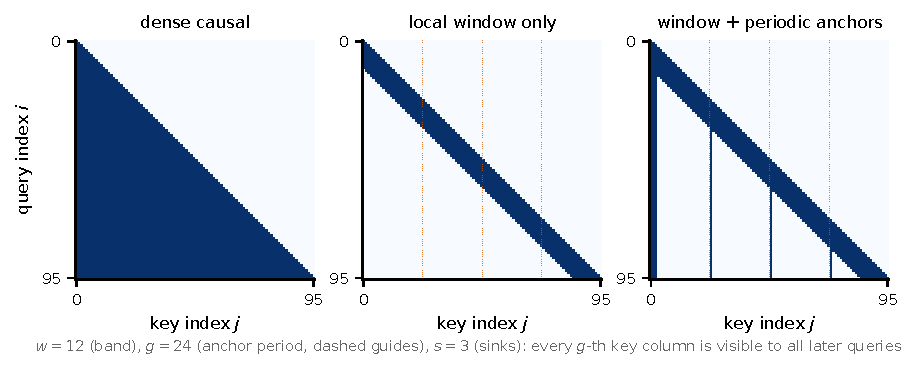
\includegraphics[width=\textwidth]{fig1_mask.pdf}
\caption{The mask family \eqref{eq:mask} at $n=96$, $w=12$, $g=24$, $s=3$. Left:
dense causal attention. Middle: a sliding window, whose global-key budget is zero.
Right: window plus periodic anchors; every $g$-th key column is visible to all
later queries, marked by the dotted guides. The third panel differs from the second
by a set of columns, not by a property of the pattern, and that set is what
Theorem~\ref{thm:linear} counts.}
\label{fig:mask}
\end{figure}

Two readings of \eqref{eq:entryasym} matter. First, the anchor term is
\emph{quadratic} in $n$: the count is $n(w+s)$ plus $(n-w)^2/(2g)$, so a fixed
period $g$ gives $\Theta(n^2)$ entries, scaled down by $1/(2g)$. The often quoted
``$\bigO(n(w+n/g))$'' is therefore linear only in the parameter, not in $n$.
Second, the two terms exchange dominance at
\begin{equation}
n^\ast \;=\; 2g\,(w+s),
\label{eq:crossover}
\end{equation}
which for the settings of Section~\ref{sec:device} is $n^\ast=\CrossoverLen$
(Figure~\ref{fig:mask} illustrates the three patterns; Figure~\ref{fig:counting}
shows the count);
below it the window term dominates and the pattern looks linear, above it the
anchor term does. At the largest length we measure, the anchors already account
for \AnchorShareAtLargestN\% of all entries while the mask retains
\DensityAtLargestN\% of the causal matrix. This is the quantitative reason why a
short benchmark suggests that a periodic-anchor design is cheap and a long one
does not.

\subsection{The linearity criterion}

\begin{theorem}[Linearity criterion]\label{thm:linear}
Consider a mask whose attended entries are a window of width $w$ plus a
global-key set of size $A(n)$ that is visible to all later queries. Then
\begin{equation}
\lvert\Sset\rvert \;=\; n\,(w+s) \;+\; \Theta\!\left(n\,A(n)\right),
\end{equation}
so the cost is $\Theta(n)$ if and only if $A(n)=\bigO(1)$, and $\Theta(n^2)$ if
$A(n)=\Theta(n)$.
\end{theorem}

The argument is a double count: each global key is attended by every later query,
hence contributes $\Theta(n)$ entries, and there are $A(n)$ of them; the window
contributes $nw$. Theorem~\ref{thm:linear} is what separates the two designs that
the literature groups under ``global attention''. A fixed global set costs
$n\lvert G\rvert$, which is linear with a constant that does not grow; a periodic
anchor set costs $n^2/(2g)$, which is quadratic however small the constant looks
at the $n$ where it was benchmarked. It also explains why a learned selection
budget that is constant per query (as in \cite{zhou2021informer}) stays in the
linear class while a coverage-driven period does not.

There is a second, harder consequence. Combining \eqref{eq:entryasym} with
Proposition~\ref{prop:block} below, the work a block-granular kernel actually
performs for the anchor term is $\Theta(n^2 B/(2g))$, i.e. the effective period is
$g/B$ blocks rather than $g$ positions. The achievable reduction relative to
dense attention is therefore bounded by $g/B$, a small constant for the anchor
periods at which the mask is at all faithful
(Corollary~\ref{cor:ceiling}).

\subsection{What a block-granular kernel actually executes}\label{sec:blocklaw}

A kernel does not execute a mask; it executes a set of $B\times B$ tiles. The
executed density is therefore a different random variable from the density of the
mask, and the difference is systematic rather than noisy.

\begin{proposition}[Granularity law]\label{prop:block}
Partition the sequence into blocks of size $B$ and let $D_{\mathrm{blk}}$ be the
fraction of causal key blocks that the pattern requires. Then
\begin{equation}
D_{\mathrm{blk}} \;=\; \min\!\left(1,\frac{B}{g}\right) \;+\; D_{\mathrm{win}},
\label{eq:blocklaw}
\end{equation}
where $D_{\mathrm{win}}$ is the diagonal band contributed by the window, and the
first term does not depend on whether $g$ is a multiple of $B$.
\end{proposition}

The first term is a counting identity: a key block of $B$ consecutive positions
contains a multiple of $g$ whenever $B\ge g$ (pigeonhole, so the term saturates at
one), and otherwise contains one with frequency $B/g$; a block that contains an
anchor is materialised even if the anchor is its only useful entry. Alignment
between $g$ and $B$ moves the anchor to the block boundary, which matters for
addressing in a streaming kernel, but it does not change how many blocks are
needed. Table~\ref{tab:block} checks \eqref{eq:blocklaw} at six settings and the
two sides agree to three decimals in all of them.

The consequence is a multiplicative inflation of the sparse work,
\begin{equation}
\frac{D_{\mathrm{blk}}}{D_{\mathrm{elm}}} \;\approx\; B
\quad\text{for } g>B,
\label{eq:inflation}
\end{equation}
because the element-level anchor density is $1/g$ while the block-level density is
$B/g$. At $B=\AlignBlock$ and $g=192$ the measured inflation is
\BlockInflationAtRef{}$\times$: a mask that is \BlockElemDensPct\% dense at element level
occupies \BlockDensCausalAtB\% of the causal blocks. The factor $B$ in
\eqref{eq:inflation} is an upper envelope, approached only once the window term
has stopped contributing to the element density; at the lengths we can measure it
still contributes, which is why the measured factor is \BlockInflationAtRef{}
rather than \AlignBlock. Equation~\eqref{eq:inflation} is the second number a
designer needs, and it is the one that the phrase ``$0.5\%$ sparse'' hides.

\subsection{The price of a cheaper mask}

Sparsity is not free in quality, and the price can be stated exactly enough to be
checked.

\begin{theorem}[Retained-mass bound]\label{thm:mass}
Let $a_i$ be the dense causal softmax distribution of query $i$, let
$\rho_i=\sum_{j\in\Sset(i)}a_{ij}$ be the mass it places on the retained set, and
let $a^{\Sset}_i$ be the renormalisation of $a_i$ onto $\Sset(i)$. For any value
matrix with $\lVert V\rVert_\infty=V_{\max}$,
\begin{equation}
\big\lVert o_i^{\mathrm{full}} - o_i^{\Sset}\big\rVert_\infty
\;\le\; 2\,(1-\rho_i)\,V_{\max}.
\label{eq:massbound}
\end{equation}
\end{theorem}

The proof is two lines of total-variation (\ref{app:proofs}) but the
bound is useful because both sides are measurable: $\rho_i$ is computable from the
dense softmax, and the left-hand side is computable by running both attention
variants. Section~\ref{sec:mass} reports the check. The theorem also explains why
the efficiency question cannot be settled on the mask alone: a mask that keeps
$16\%$ of the mass has a worst-case output error of $1.68\,V_{\max}$ before any
kernel is involved.

\begin{corollary}[Ceiling on the anchor saving]\label{cor:ceiling}
For the family \eqref{eq:mask} executed at block granularity $B$, the reduction in
attention work relative to dense attention is at most $g/B$, and the mass retained
by the same mask at length $n$ is approximately $(w+s)/n + 1/(2g)$ in count terms.
Since the retained mass decreases in $g$ while the ceiling increases in $g$, the
two objectives are in direct tension and no choice of $g$ improves both.
\end{corollary}

Corollary~\ref{cor:ceiling} is the compact statement of the design problem, and it
is the reason the measurements below come out the way they do: at $g=\GpuG$,
$B=\GpuBlock$ the ceiling is a factor of four, while the mask keeps
\RhoMean{} of the softmax mass. A designer who wants more than a factor of four
must raise $g$, and every increase buys work at the price of fidelity.

\subsection{From laws to testable hypotheses}

The theory yields seven statements, each of which the artefact marks as a
hypothesis that may come out false. They are listed with the experiment that
tests them, and Section~\ref{sec:attention} reports the verdict on each.

\begin{description}\itemsep2pt
\item[H1] Equation~\eqref{eq:entrylaw} matches the measured entry count exactly on
the grid $n\in\{256,\dots,4096\}$. (Table~\ref{tab:counting}.)
\item[H2] The local log-log exponent of $\lvert\Sset\rvert$ rises from one to two
across $n^\ast$, so a benchmark below $n^\ast$ certifies linearity that does not
hold above it. (Figure~\ref{fig:counting}.)
\item[H3] The transient memory of an anchor-based implementation grows
quadratically while the same implementation with the anchors removed grows
linearly. (Figure~\ref{fig:device}.)
\item[H4] On a memory-constrained device the anchor-based implementation is no
better than a fused dense kernel in either memory or latency at large $n$.
\item[H5] The executed block density equals $\min(1,B/g)$ plus the window term at
every measured setting. (Table~\ref{tab:block}.)
\item[H6] The retained mass is small and the bound \eqref{eq:massbound} holds with
slack. (Section~\ref{sec:mass}.)
\item[H7] A half-billion-parameter instruction-tuned model does not approach a
gradient-boosted baseline on the same rows, and adapting it on $10^2$ rows
repairs the output format without repairing discrimination.
(Section~\ref{sec:lang}.)
\end{description}

\section{Measurement protocol}\label{sec:protocol}

The claims in this paper are of a kind that is easy to state and hard to check, so
the apparatus is part of the contribution and is described before the results.
Three mechanisms do the work: unit-level provenance, a separation between claims
that must be true and claims that may be false, and an explicit refusal to
substitute estimates for measurements. The full recipe is in
\ref{app:artifact}.

\subsection{Unit-level provenance and crash-safe resume}

Each experiment is a \emph{unit} that writes exactly one JSON result file
containing the measurements, the configuration, the device, and two dictionaries:
\texttt{assertions} and \texttt{hypotheses}. A unit is marked \texttt{running}
before it starts and \texttt{done} only after its file exists and hashes to the
recorded digest; a killed process leaves \texttt{running}, which becomes
\texttt{interrupted} on the next launch and is re-executed. Completed units are
skipped by content hash. Every figure and table in this paper is generated from
these files at build time: the LaTeX source contains no typed measurement, and
the number of macros emitted by the build script equals the number of quantities
the text uses. This is what allows the sentence ``\VramPswaBig\,MiB at
$n=\LargestN$'' to be checkable rather than merely plausible.

A dependency fingerprint guards the derived layer. The figure stage records the
digests of the result files it consumed; if any upstream unit is re-run, the
digest changes, the figure unit is invalidated and regenerated. The mechanism was
added after it failed: a device benchmark was re-measured, the figure stage
reported \texttt{skipped} because its own output existed, and the repository
briefly contained a figure that did not correspond to the results beside it. A
protocol that can produce that failure silently is not adequate for a paper whose
argument is about measurement.

\subsection{Assertions versus hypotheses}\label{sec:audit}

The distinction is small and consequential. An \emph{assertion} is an internal
consistency requirement: that the mask is sparse, that the outputs are finite,
that two variants differ, that a bound holds. If an assertion is false the
artefact is broken and the run must fail. A \emph{hypothesis} is a scientific
claim: that sparsity saves memory, that a periodic anchor is supported by the
data, that adaptation helps. A hypothesis may be false, and when it is, the
correct outcome is a recorded refutation and a rewritten paper, not a failed run.

Conflating the two is not a cosmetic error. In an earlier version of this
apparatus both dictionaries were merged, so a refuted hypothesis made the
verification gate fail, and the cheapest way to a green run was to weaken the
claim until it passed. Separating them removed that incentive: the gate now
requires every assertion to be true and merely \emph{reports} the hypotheses that
came out false. Section~\ref{sec:attn_withdraw} lists what this caught in our own
work.

Two further rules apply to every unit. A measurement that could not be taken is
recorded as \texttt{blocked} with the command that would unblock it, and never
replaced by an estimate or a value borrowed from the literature. A quantity that
the pipeline could not compute, whether a parse failure, a missing class or a
degenerate split, is recorded as a failure and counted, never imputed;
Section~\ref{sec:lang} shows what imputation would have done to the headline
number of the language-model experiment.

\subsection{Device benchmark protocol}\label{sec:device_protocol}

Six decisions determine whether a memory measurement means anything, and we state
all six because three of them were wrong in our first attempt.

\begin{enumerate}\itemsep2pt
\item \emph{Baseline decontamination.} Peak memory is reported as the difference
between the maximum allocated bytes during the operation and the allocation
immediately before it, after \texttt{gc.collect()} and
\texttt{torch.cuda.empty\_cache()}, with the peak counter reset \emph{after} the
query, key and value tensors exist. Without the reset, a stale tensor inflated the
baseline by $8.5$\,MiB in our first run and produced impossible numbers at the
smallest length.
\item \emph{Two dense baselines.} We report a naive dense implementation, which
materialises the $n\times n$ score matrix, and a fused kernel
\cite{dao2022flashattention} that does not. The first is the baseline that
inflates a sparse saving; the second is the competitor a real system faces. Both
are reported for every length.
\item \emph{Two sparse implementations.} A batched variant (one gather plus one
batched matrix product per sequence, the way a production kernel would run) and a
block-streaming variant (minimal live memory, one launch per query block). The
second exists so that a memory claim cannot be dismissed as an artefact of an
inefficient gather. The two are reported separately and they behave very
differently, which is itself a result.
\item \emph{Omission is a datum.} An out-of-memory outcome is stored as
\texttt{status="oom"}, never skipped and never interpolated; the largest length at
which the dense path fails while a sparse path succeeds is reported as a measured
quantity.
\item \emph{Tail latency.} We report the median and the 95th percentile of
\GpuReps{} repetitions after warm-up, with a device synchronisation around each
repetition, because a mean over unsynchronised asynchronous launches is not a
latency.
\item \emph{Disclosure of implementation dependence.} The batched variant pads
every query block to the largest number of key blocks required by \emph{any} block
in the sequence, which is the last one. That choice is correct but not optimal,
and it inflates its memory relative to a hand-tuned kernel; we quantify the
consequence and scope the claim accordingly (Section~\ref{sec:attn_disclose}
rather than in a footnote).
\end{enumerate}

\subsection{Elicitation protocol for language models}

Two interfaces are measured on the same rows.
\emph{Logit interface}: the model is asked a yes/no question, and the score is
$p=P(\texttt{Yes})/\big(P(\texttt{Yes})+P(\texttt{No})\big)$ read at the answer
position of a single forward pass, so no text is parsed and no failure mode
exists. \emph{JSON interface}: the model is asked for a small JSON object, the
output is parsed with a regular expression, and every unparsable answer is counted
as a failure. The second interface is what practitioners do; the first exists to
separate the cost of the model from the cost of the interface.

Only the logits of the final position are computed, because materialising the full
vocabulary distribution for a batch allocates $\text{batch}\times\text{seq}\times
\lvert V\rvert$ floats and exhausts the device at the batch size we use. The
adaptation experiment replaces the hard-coded targets of the original pipeline
(which used the constants $0.90$ and $0.05$) with the per-row continuous
probability predicted by the reference model on the training split, so the target
has \TargetDistinct{} distinct values with standard deviation \TargetSd.

\subsection{Statistical protocol}

Systems are always compared on identical rows, and the comparison statistics are
paired. For a ranking metric we use a paired permutation test over rows, which
makes no distributional assumption about AUC-PR and is exact under exchangeability
\cite{efron1993bootstrap}; we report the permutation $p$-value and the observed
difference. For confidence intervals we bootstrap the difference with two
resampling units: rows, and entities (cards), because several transactions share a
card and the row unit understates the variance. The entity-level interval is the
statistically correct one and we report both so the reader can see the difference.
For paired decisions we use the exact McNemar test \cite{mcnemar1947note}, for
score differences the DeLong test \cite{delong1988comparing}, and we control the
family-wise error with Holm's step-down procedure \cite{holm1979simple}. The number
of training seeds is set by an a-priori power calculation rather than by
convention; the calculation is reported with its inputs in
\ref{app:tables}.

Calibration is reported with the Brier score and the expected calibration error
before and after Platt scaling fitted on validation only
\cite{guo2017calibration}. Fairness is reported as equalised-odds gaps
\cite{hardt2016equality} on the attributes the second dataset provides. Both are
reported even where they are unfavourable: Section~\ref{sec:system} reports a
calibration intervention that does not help and a drift comparison that is
confounded by prevalence.

\section{Results I: the counting laws hold, and the verdict reverses}\label{sec:attention}

\subsection{The entry law is exact, and linearity is an artefact of the grid}

Table~\ref{tab:counting} compares \eqref{eq:entrylaw} with the measured number of
attended entries on the grid $n\in\{256,512,1024,2048,4096\}$, with $w=\WinW$,
$g=\AnchorG$, $s=\Sinks$. The two agree at every length: the relative deviation is
\NnzLawMaxErrPct\%, i.e. the identity is exact rather than asymptotic. The
leading-order form \eqref{eq:entryasym} is also tabulated; it is the form a
designer would use, and it overstates the count by $15\%$ at $n=256$ and by
$1.2\%$ at $n=4096$, which is the size of the remainder it discards.

\begin{table}[t]
\centering
\begin{tabular}{rrrrrr}
\toprule
$n$ & measured & Eq.~\eqref{eq:entrylaw} & rel.\ err & asymptotic & density \\
\midrule
256 & 15{,}226 & 15{,}226 & +0.000\% & 17{,}600 & 46.29\% \\
512 & 33{,}370 & 33{,}370 & +0.000\% & 35{,}861 & 25.41\% \\
1{,}024 & 71{,}674 & 71{,}674 & +0.000\% & 74{,}432 & 13.66\% \\
2{,}048 & 156{,}506 & 156{,}506 & +0.000\% & 159{,}765 & 7.46\% \\
4{,}096 & 358{,}906 & 358{,}906 & +0.000\% & 363{,}200 & 4.28\% \\
\bottomrule
\end{tabular}

\caption{Entry law. Measured number of attended entries against the identity
\eqref{eq:entrylaw} and against its asymptotic form
$n(w+s)+(n-w)^2/(2g)$, with $w=\WinW$, $g=\AnchorG$, $s=\Sinks$. The identity is
exact on the whole grid, so the residual column is zero to three decimals; the
asymptotic form carries the stated remainder. The last column is the entry count as
a fraction of the causal matrix. Data:
\texttt{s1\_pswa/complexity\_curve.json}.}
\label{tab:counting}
\end{table}

The fitted log-log slope of the measured count is $\NnzSlopeFitted$ over this
grid, comfortably below the dense value of two, and it is tempting to report that
number as evidence of sub-quadratic cost. It is not, and
Figure~\ref{fig:counting} shows why. The local exponent, evaluated between
consecutive lengths, moves from $\NnzLocalExponentMin$ to $\NnzLocalExponentMax$
across the grid, because the window term still dominates below
$n^\ast=\CrossoverLen$ (Equation~\eqref{eq:crossover}); the exponent of the closed
form, extrapolated with no additional measurement, passes $1.8$ by $n=2^{15}$ and
converges to two. A benchmark that stops at $n=4096$ therefore certifies
linearity that \eqref{eq:entryasym} says cannot hold at $n=\LargestN$, and the
device measurements below are taken exactly where the crossover has been crossed.

\begin{figure}[t]
\centering
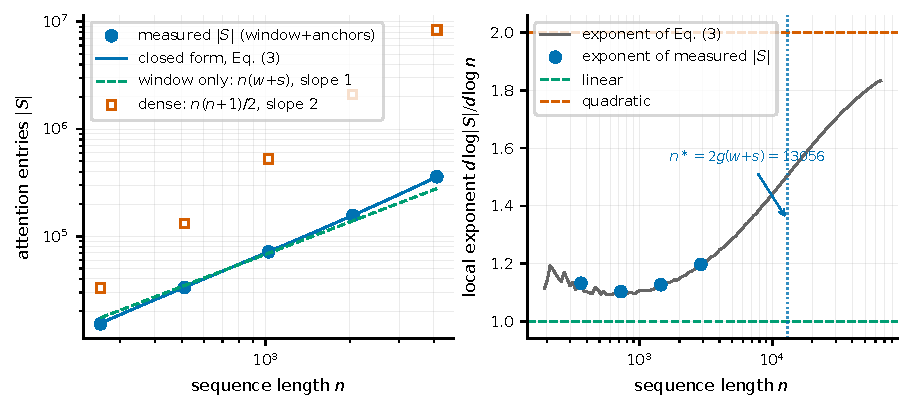
\includegraphics[width=\textwidth]{fig2_counting.pdf}
\caption{Left: attended entries against the closed form \eqref{eq:entrylaw}, the
window-only term $n(w+s)$ (slope one) and the dense count $n(n+1)/2$ (slope two).
Right: local log-log exponent of the entry count. Points are measured; the solid
curve is the exponent of the closed form, plotted beyond the measured grid to show
where it reaches the quadratic regime, and the dotted line marks the crossover
$n^\ast=\CrossoverLen$ of Equation~\eqref{eq:crossover}. The exponents of the
measured points are computed between consecutive lengths, not fitted across the
whole grid. Data: \texttt{s1\_pswa/complexity\_curve.json}.}
\label{fig:counting}
\end{figure}

\subsection{On the device, the anchor variant loses to fused dense attention}\label{sec:device}

Table~\ref{tab:device} and Figure~\ref{fig:device} report peak transient device
memory and median latency for six implementations across five orders of magnitude
of $n$, on the \GpuMemGiB\,GiB device described in Section~\ref{sec:setting}. Four
facts stand out.

\begin{table}[t]
\centering
\resizebox{\textwidth}{!}{\begin{tabular}{rrrrrrrrrrrrr}
\toprule
$n$ & \multicolumn{2}{c}{dense materialised} & \multicolumn{2}{c}{fused SDPA} & \multicolumn{2}{c}{local window} & \multicolumn{2}{c}{local + sinks} & \multicolumn{2}{c}{window + anchors} & \multicolumn{2}{c}{window + anchors, streamed} \\
 & MiB & ms & MiB & ms & MiB & ms & MiB & ms & MiB & ms & MiB & ms \\
\midrule
256 & 0.31 & 0.3 & 0.03 & 0.1 & 0.42 & 1.4 & 0.58 & 1.4 & 0.58 & 1.1 & 0.16 & 2.1 \\
512 & 1.25 & 0.3 & 0.06 & 0.1 & 0.83 & 0.9 & 1.15 & 1.1 & 1.47 & 1.2 & 0.24 & 4.7 \\
1{,}024 & 5.01 & 0.4 & 0.12 & 0.2 & 1.66 & 1.5 & 2.31 & 1.4 & 4.23 & 1.3 & 0.39 & 8.2 \\
2{,}048 & 20.02 & 0.6 & 0.25 & 0.3 & 3.33 & 1.2 & 4.61 & 1.3 & 14.20 & 1.4 & 0.69 & 16.7 \\
4{,}096 & 80.03 & 2.2 & 0.50 & 0.6 & 6.66 & 1.4 & 9.22 & 1.9 & 47.66 & 4.0 & 1.28 & 40.4 \\
8{,}192 & 320.06 & 9.6 & 1.00 & 1.0 & 13.31 & 3.0 & 18.44 & 2.2 & 178.31 & 9.0 & 2.48 & 94.9 \\
16{,}384 & 1{,}280.12 & 26.1 & 2.00 & 2.6 & 26.62 & 3.0 & 36.88 & 3.5 & 682.62 & 28.4 & 4.87 & 271.1 \\
32{,}768 & oom & - & 4.00 & 12.0 & 53.25 & 5.8 & 73.75 & 6.3 & 2{,}677.25 & 108.1 & 10.48 & 870.8 \\
\bottomrule
\end{tabular}
}
\caption{Device measurements on a \GpuName{} (\GpuMemGiB\,GiB, compute capability
\GpuCapability), float16, $d=64$, $B=\GpuBlock$, $w=\GpuW$, $g=\GpuG$, median of
\GpuReps{} repetitions. Memory is the peak transient allocation of the operator
after baseline decontamination (Section~\ref{sec:device_protocol}); \emph{oom}
marks an out-of-memory outcome that is stored as such and not interpolated.
Data: \texttt{s1\_pswa/gpu\_memory\_latency.json}.}
\label{tab:device}
\end{table}

\emph{(i) Memory grows quadratically for the anchor variants and linearly without
them.} The fitted log-log slopes of transient memory against $n$ are
\SlopeDense{} for the naive dense implementation, \SlopeSdpa{} for the fused
kernel, \SlopeSliding{} for a pure window, \SlopeLocal{} for a window plus sinks,
\SlopePswa{} for window plus periodic anchors, and \SlopeStream{} for the
streaming implementation of the same pattern. The two patterns that contain no
periodic anchors are linear; the two that contain them are not. This is
Theorem~\ref{thm:linear} observed directly. What separates the two groups is not
sparsity, since every one of these patterns attends to a vanishing fraction of the
matrix; it is whether the global-key budget is bounded.

\emph{(ii) The absolute numbers decide.} At $n=\LargestN$ the anchor variant
needs \VramPswaBig\,MiB against \VramSdpaBig\,MiB for the fused dense kernel,
i.e. $\VramTimesSdpa\times$ as much, and it is \LatencySlowdownVsSdpa$\times$
slower (\LatPswaBig\,ms against \LatSdpaBig\,ms). The naive dense path runs out of
memory at that length while the sparse path still runs. That is the one comparison
in which the sparse design wins, and it wins against the baseline a real system
would not use. Against the window-plus-sinks pattern, which is the same
family with the anchors deleted, the anchor variant costs
$\MemLocalRatio\times$ the memory and $\LatLocalRatio\times$ the latency
(\VramLocalBig\,MiB, \LatLocalBig\,ms).

\emph{(iii) Dropping the anchors improves both axes.} A pure sliding window with $w=\GpuW$ uses \VramSlidingBig\,MiB and
\LatSlidingBig\,ms at $n=\LargestN$, which is \LatSlidingRatio$\times$
\emph{faster} than the fused dense kernel and two orders of magnitude below the
anchor variant in memory. The quality cost of dropping the anchors is real and is
quantified in Section~\ref{sec:mass}; what the measurement establishes is that the
anchor machinery, as realised in an otherwise identical kernel, buys nothing on the
device and costs everything.

\emph{(iv) The streaming variant trades one pathology for another.} Processing one
query block at a time gives the asymptotically minimal live set, slope
\SlopeStream{} and \VramStreamBig\,MiB at $n=\LargestN$, and pays for it with
launch overhead: \LatStreamBig\,ms, i.e. \LatStreamRatio$\times$ the fused kernel.
The pair of sparse measurements is what makes the comparison honest: a claim of
``linear memory'' and a claim of ``practical speed'' can each be supported, but
not by the same implementation.

\begin{figure}[t]
\centering
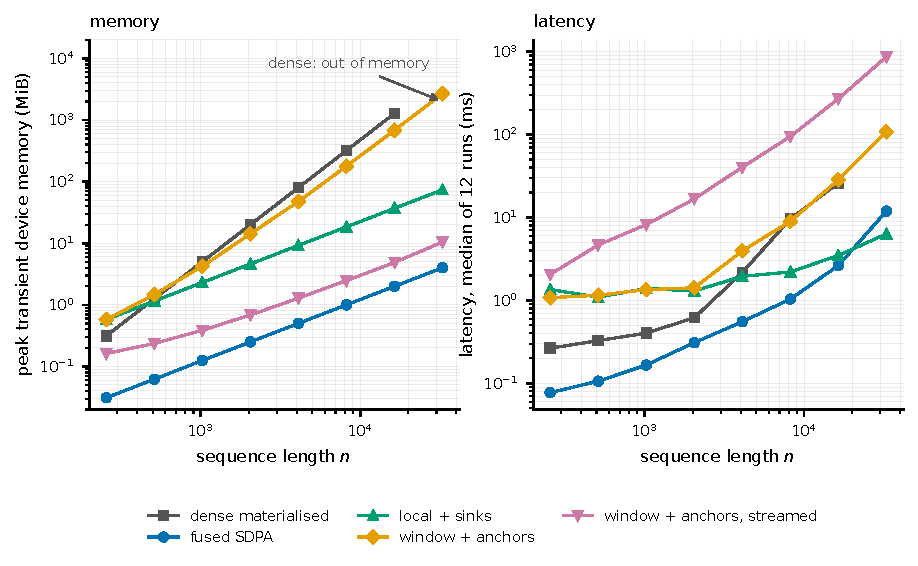
\includegraphics[width=\textwidth]{fig3_device.pdf}
\caption{Peak transient device memory (left) and median latency (right) against
sequence length, log--log, on one \GpuName{}. Slopes: dense materialised
\SlopeDense{}, fused SDPA \SlopeSdpa{}, local window \SlopeSliding{}, local plus
sinks \SlopeLocal{}, window plus anchors \SlopePswa{}, window plus anchors
streamed \SlopeStream{}. The anchor-based variants are the only ones that leave
the linear regime, and they are the only ones that lose to the fused dense kernel.
Data: \texttt{s1\_pswa/gpu\_memory\_latency.json}.}
\label{fig:device}
\end{figure}

\subsection{The kernel executes far more than the mask advertises}\label{sec:granularity}

Table~\ref{tab:block} evaluates \eqref{eq:blocklaw} at $n=\AlignN$,
$B=\AlignBlock$, $w=\AlignW$ for six anchor periods, and
Table~\ref{tab:granularity} varies the block size at a fixed period. The
decomposition is exact: the sum of the anchor term $\min(1,B/g)$ and the measured
window term reproduces the measured block density to three decimals in all six
settings, including the one where $g$ is not a multiple of $B$ and the three where
$g<B$.

\begin{table}[t]
\centering
\begin{tabular}{rrrrrr}
\toprule
$g$ & aligned & $\min(1,B/g)$ & window term & sum & measured \\
\midrule
32 & no & 1.000 & 0.000 & 1.000 & 1.000 \\
96 & no & 0.667 & 0.030 & 0.697 & 0.697 \\
128 & yes & 0.500 & 0.038 & 0.538 & 0.538 \\
192 & yes & 0.333 & 0.051 & 0.384 & 0.384 \\
256 & yes & 0.250 & 0.057 & 0.307 & 0.307 \\
512 & yes & 0.125 & 0.067 & 0.192 & 0.192 \\
\bottomrule
\end{tabular}

\caption{Granularity law \eqref{eq:blocklaw} at $n=\AlignN$, $B=\AlignBlock$,
$w=\AlignW$. The anchor term is $\min(1,B/g)$; the window term is measured; their
sum reproduces the measured block density exactly. Alignment between $g$ and $B$
does not enter the count; the ratio of executed to element density ranges from
\BlockInflationMin{} to \BlockInflationMax{} across the six periods. Data:
\texttt{s1\_pswa/block\_alignment.json}.}
\label{tab:block}
\end{table}

\begin{table}[t]
\centering
\begin{tabular}{rrrrrr}
\toprule
$B$ & aligned & block pairs & causal blocks & elements & inflation \\
\midrule
32 & yes & 10.02\% & 19.88\% & 0.540\% & 18.6$\times$ \\
64 & yes & 19.51\% & 38.41\% & 0.540\% & 36.1$\times$ \\
128 & no & 37.40\% & 72.54\% & 0.540\% & 69.3$\times$ \\
256 & no & 53.12\% & 100.00\% & 0.540\% & 98.4$\times$ \\
\bottomrule
\end{tabular}

\caption{Inflation of executed density over element density as the block size
grows at fixed period $g=192$, $n=\AlignN$, $w=\AlignW$. ``Block pairs'' is the
fraction of all block pairs the kernel materialises, ``causal blocks'' the same
count over the causal ones, and ``elements'' the fraction of the $n^2$ scores the
mask retains; inflation is the ratio of the first to the third, i.e. the factor
by which the kernel over-computes the mask. The executed density of a block
kernel is not the density of the mask it implements. Data:
\texttt{s1\_pswa/block\_alignment.json}.}
\label{tab:granularity}
\end{table}

Two consequences follow. First, one fixed mask at $g=192$, with
\BlockElemDensPct\% of the entries, occupies \BlockDensCausalAtB\% of the
causal blocks at $B=\AlignBlock$ and \BlockDensCausalSatPct\% at $B=256$: the
same mathematics, a different kernel granularity, and an inflation factor that
moves from \BlockInflationAtRef{} to \BlockInflationGranMax{} between the two
ends of the table. At the coarse end the sparse pattern is executed as dense
attention, block for block. Second, and this is the operationally useful part,
the inflation factor is predictable: it approaches $B$ for $g>B$ by
\eqref{eq:inflation}, and it saturates at $1/D_{\mathrm{elm}}$ once the block
becomes large enough that every block contains an anchor. Figure~\ref{fig:density}
shows both the exactness of the density law and the saturation of the inflation.

\begin{figure}[t]
\centering
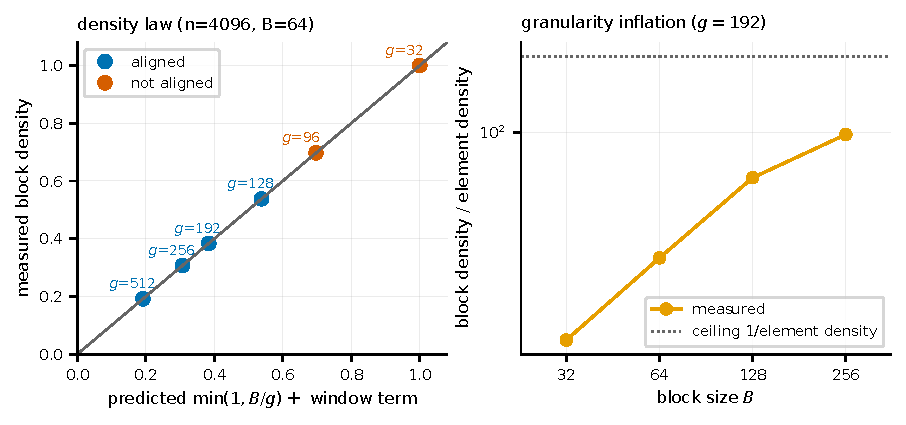
\includegraphics[width=\textwidth]{fig4_density.pdf}
\caption{Left: measured block density against the prediction
$\min(1,B/g)+$ window term; every point lies on the identity line, whether or not
the anchor period is a multiple of the block size. Right: ratio of block density
to element density against block size at fixed $g=192$; the dotted line is the
ceiling $1/$element density, reached when every block contains an anchor. Data:
\texttt{s1\_pswa/block\_alignment.json}.}
\label{fig:density}
\end{figure}

\subsection{The quality price, measured}\label{sec:mass}

Theorem~\ref{thm:mass} predicts an output deviation bounded by
$2(1-\rho)V_{\max}$. On the longest real entity sequence available in
\DatasetIeee{} we take $n=\QualityN$ ($w=\WinW$, $g=\AnchorG$, $s=\Sinks$) and
compute both sides. The mask retains $\rho=\RhoMean$ of the softmax mass on
average (minimum \RhoMin), so the deviation bound is \BoundMax{} with
$V_{\max}=\Vmax$; the measured maximum absolute output deviation is \EmpDiff, i.e.
\Tightness\% of the bound. The bound holds with slack and the slack is expected: it
is a worst-case statement over value vectors, whereas the measurement uses one
realised value matrix.

The number that matters for design is $\rho$ itself. A mask that keeps
\RhoMean{} of the mass discards $\EpsMean$ on average and up to \EpsMax{} for some
queries, and no kernel optimisation changes that: it is the geometric consequence
of a window of $\WinW$ positions on a sequence of $\QualityN$. Consistency between
this section and Section~\ref{sec:device} is not accidental: the same $w$ and $g$
are used, and the sparse implementation there is the implementation whose
deviation is bounded here.

\subsection{The data do not contain the period the mask assumes}\label{sec:acf}

The periodic anchor is only a modelling choice if some periodicity exists. We
therefore estimate the autocorrelation function of the real entity sequences
directly, on the \NSequences{} longest sequences, up to lag $200$. The spectrum is
dominated by short-range dependence: the lag-1 coefficient is \AcfLagOne, lag 2 is
roughly half of it, and the decay continues monotonically. There is a weak local
bump at lag \AcfWeakLag{} (\AcfWeakPeak), but it sits inside the tail of that decay
rather than above it. In the band around the period actually used,
$[\AnchorBandLo,\AnchorBandHi]$, the largest coefficient is at lag 65 and the
coefficient at $g=\AnchorG$ itself is \AcfAtG{} against a high-lag noise floor of
\AcfNoiseFloor{}: no periodic peak is significant.

The consequence is a scope condition, not a refutation of the mask. We use
$g=\AnchorG$ in every controlled experiment as a \emph{pre-registered control},
not as a learned parameter, and the artefact records
\texttt{g\_is\_data\_driven = false} beside those results. Anyone who reads the
device measurements as ``this period is right for this data'' would be
over-reading them; the measurements are about the cost of the pattern, and the
cost is the same for any period of the same size.

\subsection{Verdict, and what part of it is our implementation's fault}\label{sec:attn_disclose}

H1, H2, H3, H5 and H6 hold. H4 holds: on this device the anchor-based
implementation is worse than the fused dense kernel in both memory and latency at
every length where both run. We are careful about what H4 does and does not mean.

The measured cost of the anchor variant is the product of three factors: the
counting law (Prop.~\ref{prop:count}), the granularity inflation
(Prop.~\ref{prop:block}, measured at \BlockWorkInflation{}$\times$ the element
count at $B=\GpuBlock$ and $g=\GpuG$, i.e. between $B/2$ and $B$ while the window
term still contributes), and a padding factor of \PadFactor{} in our
batched kernel, which pads every query block to the
\MaxSelBlocks{} key blocks required by the last block instead of the
\MeanSelBlocks{} it needs on average. A hand-tuned kernel can remove the third
factor and part of the second, and we say so: the first two remain, and they are
properties of the family rather than of our code. Concretely, dividing the
measured memory and latency at $n=\LargestN$ by the padding factor leaves
\VramAfterDepad\,MiB and \LatAfterDepad\,ms, still far above the fused kernel's
\VramSdpaBig\,MiB and \LatSdpaBig\,ms. The ceiling of Corollary~\ref{cor:ceiling}
then bounds what any such kernel could achieve: a factor of $g/B=4$ at these
settings, against a mask that already keeps only \RhoMean{} of the mass.

We therefore scope the claim precisely. We do not claim that anchor-based sparsity
is asymptotically inferior to dense attention in arithmetic; we claim that (a) the
family is quadratic in the sequence length for any fixed period, (b) its arithmetic
advantage over dense attention is bounded by $g/B$, and (c) on a memory-constrained
device, with the implementation a practitioner would write from the published
description, it is dominated by a fused dense kernel at every length that device
can hold, while the same pattern without anchors is not. Claim (a) is proved,
claim (b) follows from the counting law and the granularity law, and claim (c) is
measured.

\subsection{A claim of ours that the apparatus refuted}\label{sec:attn_withdraw}

An earlier version of this work asserted a \emph{block-alignment lemma}: that
block-level sparsity requires the anchor period to be a multiple of the block
size, and that otherwise the pattern ``degenerates towards dense''. The claim was
false, and the way it failed is instructive enough to report.

The assertion that carried it compared the largest block density among unaligned
periods with twice the smallest among aligned ones. That is, it compared
\emph{different} values of $g$. On a steep grid the comparison is won by
construction, and the assertion held for reasons unrelated to the claim. The data
contradict it directly. At $B=\AlignBlock$ the aligned period $g=192$ gives a
block density of \WithdrawDensAligned{}, the unaligned period $g=96$ gives
\WithdrawDensUnaligned{}, and the densest row in the grid, $g=32$ at
\WithdrawDensDensest{}, is not a multiple of the block size at all. Density
tracks $g$, not alignment: a longer period is sparser whether or not it divides
the block size, and the densest row in the grid comes from $g<B$, which is a
different mechanism altogether. What survives is
\eqref{eq:blocklaw}: alignment does not change how many blocks are needed, it only
places the anchor on a block boundary, which matters for address arithmetic in a
streaming kernel and for nothing else.

We replaced the lemma with the counting law, re-ran the unit, and kept the flag
\url{former_lemma_withdrawn} in the result file so that a reader of the
artefact can see both versions. Section~\ref{sec:audit} explains why the apparatus
let a false claim through in the first place: the assertion and the hypothesis had
been merged, so the claim was encoded as something that had to be true.

\section{Results II: the small language model is supervision-bound}\label{sec:lang}

\subsection{What the interface costs}

The same \LlmRows{} held-out transactions (\LlmPositives{} positives) are scored
twice by the same \num{0.5}-billion-parameter instruction-tuned model
\cite{qwen2024report}, once through the logit interface and once through generated
JSON. Reading the answer as a probability costs \LlmMsRow\,ms per row
(\LlmRowsPerS{} rows/s); generating and parsing a JSON object costs
\JsonMsRow\,ms per row (\JsonRowsPerS{} rows/s). The interface alone accounts for
a factor of \InterfaceRatio{} in latency, more than the difference between the two
model sizes we measure in Section~\ref{sec:scale} and more than most architecture
choices a practitioner would deliberate over. The cost sits in the interface, not
in the model.

The JSON interface also fails, completely. All \ParseFailRows{} of
\ParseFailDenom{} attempts were unparsable, and the failures are not random: the
model answered conversationally, with the same preamble every time, for example
``\emph{No. This transaction appears to be legitimate, as it includes all required
fields \dots}''. Every failure therefore maps to the same constant, the score
distribution collapses to a single value, and any ranking metric computed on the
imputed fallback would be measuring the fallback rather than the model. The
original pipeline of this project did exactly that, substituting $0.9$ or $0.1$
depending on the surface form of the failure. We record the failures and report
them; the discrimination numbers below use the logit interface, which has nothing
to parse.

\subsection{Zero-shot discrimination}

\begin{table}[t]
\centering
\resizebox{\textwidth}{!}{\begin{tabular}{lrrrrrr}
\toprule
system & AUC-PR & AUC-ROC & R@FPR$=1\%$ & F1 & parse fail & ms/row \\
\midrule
GBDT, same rows & 0.5295 & 0.9053 & 35.5\% & 0.4356 & -- & -- \\
0.5B, logit interface & 0.0767 & 0.6412 & 4.8\% & 0.0750 & 100.0\% & 6.3 \\
0.5B, JSON interface & -- & -- & -- & -- & 100.0\% & 139.5 \\
0.5B + LoRA (900 rows) & 0.0364 & 0.4582 & 0.0\% & 0.0000 & 0.0\% & 7.8 \\
\bottomrule
\end{tabular}
}
\caption{Language model against gradient-boosted trees on identical held-out rows.
The logit interface reads $P(\texttt{Yes})$ at the answer position; the JSON
interface generates and parses an object. Parse failures are counted, never
imputed. Latency is per row in the same run. Data:
\texttt{s8\_llm/zero\_shot\_0\_5b.json},
\texttt{s8\_llm/lora\_sft\_0\_5b.json}.}
\label{tab:llm}
\end{table}

Table~\ref{tab:llm} reports the comparison. The model is not at chance: AUC-ROC
\LlmAucRoc{} and AUC-PR \LlmAucPr{} against a base rate of
$\LlmPositives/\LlmRows\approx 4.1\%$ show that it extracts some signal from the
serialised row. But the gradient-boosted model on the same rows reaches AUC-PR
\GbdtSameAucPr{} and AUC-ROC \GbdtSameAucRoc{}, and the paired difference is
\LlmDelta{} with a row-level bootstrap interval of
\LlmCiLo--\LlmCiHi{} and a permutation $p<10^{-3}$. At the auditable operating
point, recall at a $1\%$ false-positive rate, the gap is
\LlmRecall\% against \GbdtSameRecall\%. The claim that a locally hosted model of
this size comes within two points of the tabular baseline is therefore refuted at
this scale, and the artefact records the corresponding flag as false.

\begin{figure}[t]
\centering
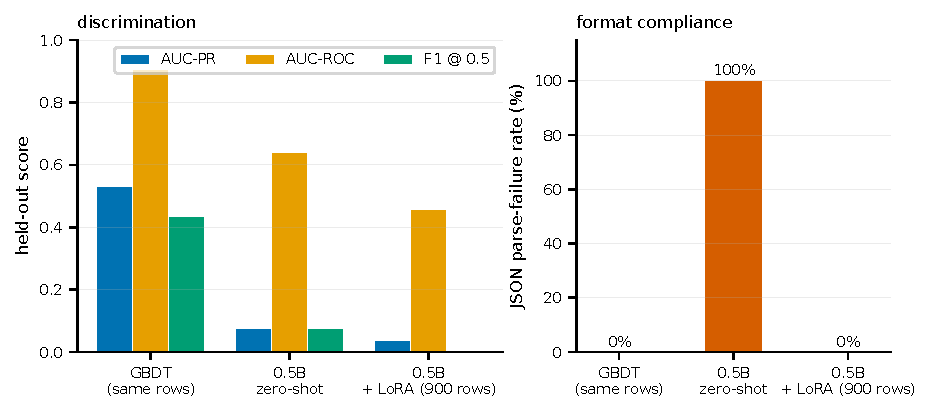
\includegraphics[width=\textwidth]{fig5_llm.pdf}
\caption{Left: held-out AUC-PR, AUC-ROC and $F_1$ for the tabular baseline and two
variants of the language model. Right: rate of unparsable JSON answers. Adaptation
moves the right panel from complete failure to complete success while moving the
left panel in the wrong direction. Data: \texttt{s8\_llm/*.json}.}
\label{fig:llm}
\end{figure}

\subsection{Adaptation repairs the format and destroys the discrimination}

LoRA \cite{hu2022lora} is applied to the query, key, value and output projections
($r=8$), giving \SftTrainable{} trainable parameters, \SftTrainablePct\% of the
model. The training set is \SftRows{} rows with per-row continuous targets: the
supervised baseline's predicted probability for that row, with mean \TargetMean,
standard deviation \TargetSd{} and \TargetDistinct{} distinct values in
$[\TargetMin,\TargetMax]$. The target therefore carries the difficulty of each row
instead of a constant. Training
takes \SftSeconds\,s on the same device, reaching a loss of \SftLoss{} with
\SftVram\,GiB peak memory.

The result is a clean dissociation, and it is the sharpest evidence in this paper
(Table~\ref{tab:llm}, right-hand rows, and Figure~\ref{fig:llm}). The parse-failure
rate goes from \ParseFailZero\% to \SftParseFail\%: adaptation teaches the output
convention perfectly. At the same time AUC-PR falls from \LlmAucPr{} to
\SftAucPr{} ($\Delta=\SftDelta$) and AUC-ROC falls from \LlmAucRoc{} to
\SftAucRoc, i.e. to chance; $F_1$ at a $0.5$ threshold goes to \SftFOne{} because
the adapted model stops emitting positive answers altogether.

We read this as an identification rather than a curiosity. Two properties of the
system used to change together, format compliance and decision quality, and the
literature on prompting and adaptation usually reports them as one number. By
measuring them separately we can say which one the update moved. \SftRows{}
labelled rows are enough to teach a syntax and not enough to teach a boundary; the
degradation is therefore evidence about supervision, not about the adaptation
method, which did exactly what it was asked. The corollary for practice is
uncomfortable: with a small labelled set, an adapted language model can look
\emph{more} usable (it answers in the requested format) while being \emph{less}
useful (it ranks worse than the prompt it replaced).

\subsection{Two model sizes, and why we stop there}\label{sec:scale}

We measure a second size, \LargeParams{}B parameters, on a \ScaleRows-row subset:
\LargeVram\,GiB peak memory and AUC-PR \LargeAucPr, against \SmallVram\,GiB and
\SmallAucPr{} for the \SmallParams{}B model. The larger model is not better on this
task; with two points we cannot distinguish a genuine inverse-scaling effect from
noise in a \ScaleRows-row evaluation, and we do not try. What the two points do support
is a memory statement: peak memory grows at \ScaleSlope\,GiB per billion
parameters, so a $7$B model at this precision would need roughly four times the
\GpuMemGiB\,GiB of the device under test. Extrapolating further would be a model of
our own making, not a measurement, and the artefact labels it as a two-point fit.
The scale question a reviewer will ask, whether the gap closes at $7$B or $8$B,
is left open, with the command that would answer it in \ref{app:artifact}.

\subsection{Verdict}

H7 holds. A half-billion-parameter model is an order of magnitude behind
gradient-boosted trees in AUC-PR on identical rows, its interface choice costs a
factor of \InterfaceRatio{} in latency, its generative interface fails on every
row, and adaptation on $10^2$ rows moves the format and the discrimination in
opposite directions. None of this says that language models cannot make tabular
decisions; it says that at this size and this supervision budget the substitution
is not neutral, and that the two failure modes must be measured separately to see
which one is binding.

\section{Results III: the decision system under a cost criterion}\label{sec:system}

The two laws above constrain the components; this section reports the system they
were meant to serve, so that the efficiency questions are anchored to a decision
problem rather than to a benchmark.

\subsection{Supervised baselines and the cost of a second stage}

\begin{table}[t]
\centering
\begin{tabular}{lrrrrr}
\toprule
system & AUC-PR & AUC-ROC & R@FPR$=1\%$ & loss & cost/tx \\
\midrule
linear (logistic) & 0.1874 & 0.7573 & 14.0\% & 9{,}299 & 1.00 \\
GBDT gate & 0.4551 & 0.8664 & 38.6\% & 6{,}653 & 1.00 \\
GBDT strong & 0.4691 & 0.8734 & 40.2\% & 6{,}580 & 20.00 \\
cascade (gate+strong) & 0.4711 & 0.8729 & 39.5\% & 6{,}552 & 19.08 \\
\bottomrule
\end{tabular}

\caption{Held-out performance on \DatasetIeee{} with \MainFeatures{} predictors,
\MainTrainRows{} training rows and \MainTestRows{} test rows. The operating point
is chosen once on validation at a $1\%$ false-positive rate. Cost per transaction
is a proxy counting the second stage as twenty times the first, not a measured
latency. Data: \texttt{s5\_baselines/main\_table.json}.}
\label{tab:main}
\end{table}

Table~\ref{tab:main} reports \Nsys{} systems. The linear model reaches AUC-PR
\AucPrLinear, the gradient-boosted gate \AucPrGbdt, a stronger gradient-boosted
second stage \AucPrStrong, and the cascade \AucPrCascade. The cascade buys
$+\PermDeltaCvG$ AUC-PR over the gate alone at a proxy cost of \CostCascade{}
against \CostStrong{} for running the strong model on everything, with an upgrade
rate of \UpgradeRate\%. The gain is small but not attributable to noise: the paired
permutation test gives $p<10^{-3}$ and the entity-cluster bootstrap interval
excludes zero (\PermCiLoCvG--\PermCiHiCvG), while the recall-at-$1\%$-FPR interval
includes zero, so the ranking improvement does not translate into a better
operating point. We report both.

The comparison that matters statistically is the one between the linear model and
the gate: $\Delta$AUC $=\DelongDelta$ (95\% CI \DelongCiLo--\DelongCiHi,
$z=\DelongZ$), with \McNemarDiscordant{} discordant pairs under McNemar
($b=\McNemarB$, $c=\McNemarC$, $p=\McNemarP$). Across \SeedN{} independent
retraining seeds the gate's AUC-PR is \SeedMean$\pm$\SeedSd, and the a-priori
power calculation says that \RequiredSeeds{} seeds would be needed to resolve a
difference of the size we observe at $80\%$ power. We therefore report the effect
size and the interval rather than a bare $p$-value, and we do not claim a
difference between systems whose intervals overlap.

\subsection{Cost sensitivity}

\begin{table}[t]
\centering
\begin{tabular}{rrrrr}
\toprule
$c_{\mathrm{FN}}/c_{\mathrm{FP}}$ & threshold & cost/tx & recall & FPR \\
\midrule
1 & 0.3058 & 0.0292 & 33.5\% & 0.58\% \\
2 & 0.2322 & 0.0527 & 38.3\% & 0.93\% \\
5 & 0.1531 & 0.1208 & 42.5\% & 1.95\% \\
10 & 0.0800 & 0.2124 & 54.5\% & 5.27\% \\
20 & 0.0370 & 0.3803 & 67.9\% & 15.79\% \\
50 & 0.0195 & 0.6403 & 79.4\% & 28.55\% \\
100 & 0.0096 & 0.7917 & 92.3\% & 53.57\% \\
\bottomrule
\end{tabular}

\caption{Cost sensitivity on \DatasetIeee{} test rows. The threshold is chosen on
validation for each cost ratio and applied once to test. Data:
\texttt{s4\_stats/cost\_sensitivity.json}.}
\label{tab:cost}
\end{table}

Table~\ref{tab:cost} and Figure~\ref{fig:cost} sweep the ratio
$c_{\mathrm{FN}}/c_{\mathrm{FP}}$ from $1$ to \CostRatioMax{} and re-select the
threshold on validation each time. Expected cost per transaction rises from
\CostAtOne{} to \CostAtHundred{} as the ratio increases, which is expected: a
higher relative cost of a missed fraud buys recall with false alarms, and recall
moves from \RecallAtOne\% to \RecallAtHundred\% while the false-positive rate moves
to \FprAtHundred\%. The useful observation is that the threshold responds smoothly
and monotonically, so the deployed operating point can be audited against a stated
cost ratio instead of being fixed by convention. It also makes the insufficiency of
a single number concrete: the same model is a different system at ratio $1$ and at
ratio $100$.

\begin{figure}[t]
\centering
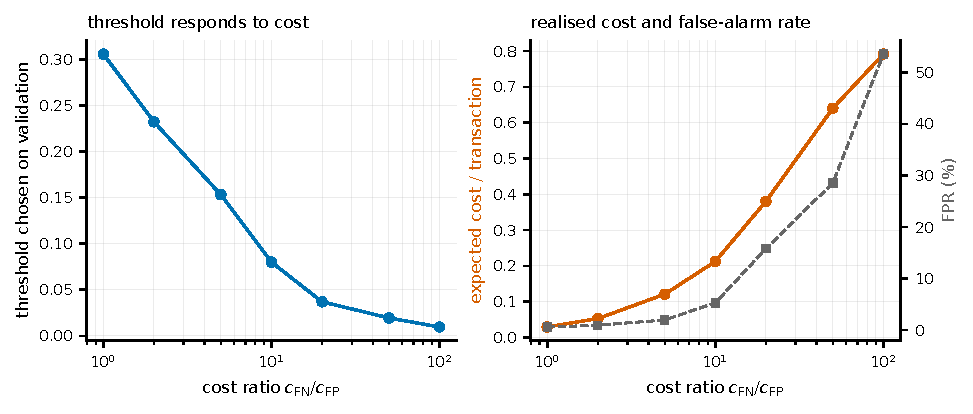
\includegraphics[width=\textwidth]{fig6_cost.pdf}
\caption{Threshold selected on validation (left) and realised test cost with the
false-positive rate (right) as the relative cost of a missed fraud increases. Data:
\texttt{s4\_stats/cost\_sensitivity.json}.}
\label{fig:cost}
\end{figure}

\subsection{Where the model transfers, and where it does not}

On \DatasetBaf{} the same pipeline with \BafFeatures{} predictors reaches AUC-PR
\BafAucPr{} and AUC-ROC \BafAucRoc{} at \BafRecall\% recall at a $1\%$ false-positive
rate. We report the number without enthusiasm and with two caveats. The dataset is
source-declared synthetic, so this is a transfer check rather than external
validation; and its base rate is lower than \DatasetIeee{}'s, so the two AUC-PR
values are not directly comparable.

Within the held-out periods of \DatasetIeee{} the AUC-PR moves by \IeeeDrift{}
between the first and last temporal slice, i.e. it is essentially flat. On
\DatasetBaf{} it moves by \BafDrift{}, and the move is confounded: the fraud
prevalence rises from \BafPrevLo\% to \BafPrevHi\% over the same interval, and
AUC-PR is prevalence-sensitive. We therefore do not interpret the second number as
evidence of improving robustness, and we record the confound rather than the
headline.

Fairness is reported as equalised-odds gaps \cite{hardt2016equality} over the
\FairAttrs{} attributes the dataset provides. The largest true-positive-rate gap
is \FairTprGap{} on \texttt{\FairAttr} across \FairGroups{} groups, with a
false-positive-rate gap of \FairFprGap; the smallest true-positive-rate gap among
the attributes is \FairMinTprGap. These gaps are a property of a single threshold
on a single dataset and we make no claim about their cause.

\subsection{Two interventions that did not help}

Calibration is the standard remedy for scores that are used as probabilities.
Fitting Platt scaling on validation and evaluating on test moves the Brier score
from \BrierPre{} to \BrierPost{} and the expected calibration error from \EcePre{}
to \EcePost; the intervention does not reduce the Brier score
(\texttt{platt\_reduces\_brier}, whose value here is \PlattImproves). The
gradient-boosted scores were already close to calibrated at this operating point,
so the honest report is a null result, and we keep it rather than dropping the
comparison.

The learning curve over labelled-set sizes from the smallest to the largest size
we evaluate moves AUC-PR from \CurveSmallAucPr{} to \CurveLargeAucPr{} across
\CurveSizes{} sizes. At the smallest size a minority floor has to be enforced,
because a uniform draw at a $3.5\%$ rate contains no positive example at all, so
the left end of the curve is an artefact of the apparatus rather than a scientific
finding.
We report the artefact because a crossover claim at that size would otherwise look
like a result. The field ladder from \LadderSmall{} to \LadderLarge{} fields moves
AUC-PR from \LadderSmallestAucPr{} to \LadderLargestAucPr, which is the expected
saturating shape and confirms that the feature budget used elsewhere in the paper
is not the binding constraint.

\subsection{What verifiability costs}

If a decision must be auditable, the audit itself has a cost, and it is fair to
state it in the same currency as the rest. A commitment-and-challenge protocol
commits to each decision, anchors a batch root, and answers a random challenge by
recomputation. We compile a registry contract with \SolcVer{} and execute it on a
local EVM: one per-transaction log commitment costs \GasPerTx{} gas (standard
deviation \GasPerTxSd), one batch root costs \GasBatch, and verifying one inclusion
proof of depth \MerkleDepth{} costs \GasVerify. Anchoring \GasBatchSize{}
transactions in one root instead of individually reduces the anchoring cost by
\GasSavingPct\%. Deployment costs \GasDeploy{} gas and is amortised.

Two limits are stated rather than papered over. First, this is a local EVM: the
numbers are receipts from executed transactions rather than a public-network
market quote, and the pricing constants are labelled as reference values that
rescale the dollar figure linearly. Second, the soundness argument for the
challenge protocol is game-theoretic, not hardware-rooted: the escape probability
of an adversary who cheats on a fraction $f$ of records falls geometrically in the
challenge rate, and a predictable challenge source destroys the guarantee
entirely. Hardware attestation \cite{costan2016sgx} and proof-of-learning
\cite{jia2021proof} would replace that assumption. Neither is measurable on this
device: the attestation unit is recorded as blocked, with the command that would
unblock it, and the proof-carrying variant was not attempted for the same reason.
We estimate neither, and no number in this paper depends on them.

\section{Discussion}\label{sec:discussion}

\subsection{Three counts, and why they belong together}

The two halves of this paper look unrelated. One is about attention kernels, the
other about language models applied to tabular rows. The argument is the same in
both. A substitution justified by an adjective (``sparse'', ``pretrained'') is
replaced by a substitution justified by a count, and the count is checked before
the adjective is trusted. For attention the counts are the global-key budget
$A(n)$ of Definition~\ref{def:budget} and the granularity inflation $B/g$ of
Proposition~\ref{prop:block}; for the language model the count is the number of
labelled rows per decision class. Each is a small integer or a simple ratio,
available before training, and in our experiments each predicts the sign of the
result.

The counts also explain \emph{why} the defaults are attractive, which matters for
anyone trying to change practice. Each default removes something awkward to
obtain, namely a task-specific global-token set, a kernel written by hand for one
pattern, or a labelled dataset, and puts something cheap in its place. Under the
constraint that produced it, the substitution is rational. What the measurements
add is the price list. The awkward quantity is worth something, and the cheap
substitute can be an order of magnitude worse on the device, or in the metric the
deployment actually uses.

\subsection{On reporting refutations}

Three claims of our own were refuted during this work and all three are reported
here: the periodicity of real entity sequences
(Section~\ref{sec:acf}), the block-alignment lemma
(Section~\ref{sec:attn_withdraw}), and the premise that a small locally hosted
model comes within two points of a tabular baseline (Section~\ref{sec:lang}). A
fourth, the claim that a sparse pattern saves device memory and latency, survives
only against a baseline that no real system would use, and we say so instead of
quoting the favourable comparison (Section~\ref{sec:attn_disclose}).

We report them because the alternative is worse for the field. Anecdotally, the
failure mode of applied efficiency work is not fabrication but attrition: the
comparison against the naive baseline is kept, the comparison against the fused one
is dropped, the run that produced a null result is not reported, and the paper that
emerges is internally consistent and externally useless. The protocol of
Section~\ref{sec:audit} is a defence against attrition that does not depend on the
author's discipline at the moment of writing: a hypothesis that came out false is a
first-class object in the result file, and the paper has a place to put it.

\subsection{Practical guidance}\label{sec:guidance}

The following procedure is what we would recommend to a team about to adopt either
default, and it is short enough to be used before a project starts.

\begin{enumerate}\itemsep2pt
\item \textbf{Write the mask's entry count, not its complexity class.} Compute
$\lvert\Sset\rvert$ as a function of $n$ for the lengths you will actually serve.
If the count contains a term $n^2/g$ with a fixed $g$, the pattern is quadratic and
the adjective ``sparse'' is describing a constant factor.
\item \textbf{Compute the global-key budget.} If the number of keys visible to
every query grows with $n$, the pattern cannot be linear. Cap the budget first, and
choose the pattern afterwards.
\item \textbf{Divide by the block size.} The executed density is
$\min(1,B/g)$ plus the window term; multiply by $B/B$ to obtain what the kernel
will actually touch. A pattern that is cheap at element granularity can be
expensive at tile granularity.
\item \textbf{Compare against the fused baseline, and against the no-anchor
variant.} The first tells you whether the pattern beats what a real system runs;
the second tells you whether the anchors you added are worth their cost. In our
measurement the second comparison is the one that decides the question.
\item \textbf{Separate interface from model.} When a language model is used as a
decision maker, measure the parse-free interface and the generative one on the same
rows; the difference is often larger than the difference between models, and only
one of the two has a failure mode.
\item \textbf{Count the rows.} Before adapting, state how many labelled examples
per class are available. If the answer is in the hundreds, expect the adaptation to
change the format and not the boundary, and measure both.
\end{enumerate}

\subsection{Threats to validity}

\paragraph{Internal} Splits are strictly temporal and never shuffled; all
fit-dependent statistics are fitted on the training partition only; the operating
point is selected on validation and applied to test once; every comparison between
systems uses identical rows. The two places where internal validity is weakest are
the field ladder, whose smallest sizes require a minority floor, and the
two-point scale fit, which we decline to extrapolate.

\paragraph{Construct} AUC-PR is the primary ranking metric because the positive
class is rare, and it is prevalence-sensitive, which is why we refuse to read the
\DatasetBaf{} drift as robustness. Verifiability is operationalised as an escape
probability under a random challenge, not as a hash-match rate; privacy is not
measured at all beyond the entropy of the salt. Cost per transaction for the second
stage is a proxy constant, not a measured latency, and is labelled as such wherever
it appears.

\paragraph{External} Two datasets, one of them synthetic, and the real one is a
single competition dataset whose slices are not independent external validation.
The entity key is \texttt{card1} because the mirror's user identifier is entirely
null, so entity grouping is coarser than the source intends. One device, one GPU
architecture, one block size, one window. All measurements are single-run except
where seeds or repetitions are reported, and we report repetitions everywhere the
number is a latency.

\paragraph{Conclusion} Ten independent training seeds, clustered and time-block
bootstraps, Holm correction across the two primary tests, effect sizes and an
a-priori power calculation. Where an interval includes zero we say that the
difference is not established, even when the point estimate is favourable.

\paragraph{Hardware and scope} TEE attestation, proof-carrying inference, a
$7$B-class full-precision baseline and public-network gas are not measured. They
are listed with the command that would unblock them and no estimate is substituted.
The quantitative claims of this paper are therefore scoped to a
\GpuMemGiB\,GiB device and a local EVM. The qualitative claims, the two laws, are
scoped only by their hypotheses, which are stated in the theorems.

\subsection{What this work does not establish}

Nothing here establishes that anchor-based sparsity is useless in general. A
fused implementation that materialises the anchor term once per batch, a hardware
pattern able to address strided key blocks without a gather, or a workload whose
$n$ sits far beyond the crossover could each change the verdict, and
Corollary~\ref{cor:ceiling} says how much room there is: a factor of $g/B$, four
at our settings. Nor is there a scale law for language models. Two sizes are two
points, and the inverse ordering at $600$ rows is as likely to be evaluation noise
as an effect. Finally, the decision systems of Section~\ref{sec:system} are not
offered as close to the best achievable on these datasets. Their feature and row
budgets are deliberately small, and a better tabular model would widen the gap
reported in Section~\ref{sec:lang}.

\subsection{Relevance to the wider AI audience}

We close where Section~\ref{sec:intro} began. The two substitutions studied here
are instances of a general move in applied AI: replace an expensive, structured
component by a cheap, general one, and justify it with a scaling argument. The
move is often right. When it is wrong, it is usually wrong for a reason that can be
counted before the experiment, and the count is the part that does not get
published. Our contribution is to make three of those counts explicit, prove them
where they can be proved, measure them where they cannot, and leave the
contradictions in the record. If the reader takes one thing from the paper, we
would prefer it to be the procedure in Section~\ref{sec:guidance}: write the
count first, and let it choose the architecture.

\section{Conclusion}\label{sec:conclusion}

We set out to check two defaults that are usually assumed. For attention we gave
an entry law that is exact to the last attended entry, a linearity criterion that
separates sparse patterns with a bounded global-key budget from those whose budget
grows with the sequence, and a granularity law that predicts how much of the
advertised sparsity survives contact with a block kernel. On a
\GpuMemGiB\,GiB device these laws predict, and the measurements confirm, that a
periodic-anchor pattern needs $\VramTimesSdpa\times$ the transient memory of fused
dense attention and is \LatencySlowdownVsSdpa$\times$ slower at
$n=\LargestN$, while the same pattern with the anchors removed is linear and
\LatSlidingRatio$\times$ faster. A global-key budget that grows with the sequence
is quadratic by construction, and no kernel trick changes the class.

For language models we separated the interface from the model, and the format from
the decision. Reading an answer as a probability instead of parsing generated JSON
is \InterfaceRatio$\times$ cheaper and cannot fail to parse; the generative
interface failed on every row we tried. On identical rows a half-billion-parameter
model trails gradient-boosted trees by \LlmDelta{} AUC-PR, and adapting it on
\SftRows{} rows repairs the output format completely while driving AUC-ROC from
\LlmAucRoc{} to \SftAucRoc. What binds is the number of supervision rows, and the
dissociation only becomes visible when the two effects are measured apart.

Behind both results sits a protocol in which claims carry a status, refuted
hypotheses stay in the record, blocked measurements are listed rather than
estimated, and every number in the manuscript is regenerated from a stored result
file at build time. It refuted three of our own claims during this work, and we
report them. The lesson is narrower than ``these defaults are bad''. A
substitution justified by a scaling argument should be justified by the count, and
the count is cheap. Write it first.


\appendix
\section{Proofs}\label{app:proofs}

\subsection*{Proposition~\ref{prop:count} (entry law)}

Fix a query $i$ and write $W_i=\{j: i-w<j\le i\}$ for the window,
$S_i=\{j:j<s,\ j\le i\}$ for the sinks and
$K_i=\{j: j\le i,\ j\bmod g=0\}$ for the anchors. All three sets are intersected
with $j\ge 0$.

\emph{Case $i<w$.} Then $W_i=\{0,\dots,i\}$, so $S_i\subseteq W_i$ and
$K_i\subseteq W_i$; hence $\lvert\Sset(i)\rvert=i+1$, and the first $w$ rows
contribute $\sum_{i=0}^{w-1}(i+1)=w(w+1)/2$.

\emph{Case $i\ge w$.} Now $W_i=\{i-w+1,\dots,i\}$ and $\lvert W_i\rvert=w$. The
sinks lie below the window, and the two sets are disjoint once
$i-w+1>s-1$, i.e. $i\ge w+s-1$; for the intermediate rows the disjoint part is
$\min(s,\,i-w+1)$ entries. The anchors that are not already counted in $W_i$ are
those with $j\le i-w$, and among them those with $j<s$ coincide with $S_i$; when
$s\le g$ the only multiple of $g$ below $s$ is $0$, so the number of new entries is
$\lfloor (i-w)/g\rfloor$ for $i\ge w$. Summing the three contributions gives
\eqref{eq:entrylaw}. The asymptotic form follows because
$\sum_{i=w}^{n-1}\lfloor (i-w)/g\rfloor = \frac{(n-w)^2}{2g}+\bigO(n)$ and the
remaining sums are $n(w+s)$ up to $\bigO(1)$. All experiments in this paper use
$s=\Sinks\le\min(w,g)$, so the side condition is satisfied. $\square$

\subsection*{Theorem~\ref{thm:linear} (linearity criterion)}

Let the global-key set be $G(n)$ with $\lvert G(n)\rvert=A(n)$, and let each
$j\in G(n)$ be visible to every query $i\ge j$ and to no query $i<j$ (causality).
If $j\notin W_i$ the key contributes one entry to row $i$ for each
$i\ge j+w$, so the total contribution of that key is $n-j-w+o(n)$, and summing over
$G(n)$ gives
\[
\sum_{j\in G(n)} (n-j) \;=\; n\,A(n) \;-\; \sum_{j\in G(n)} j .
\]
For a set spread over the sequence the second sum is
$\Theta\!\big(nA(n)\big)$, and for the periodic set $G(n)=\{0,g,2g,\dots\}$ it is
$g\frac{A(n)(A(n)-1)}{2}$, so the contribution is
$nA(n)-\frac{g}{2}A(n)^2$ with $A(n)=\lceil n/g\rceil$, which equals
$\frac{n^2}{2g}+\bigO(n)$ and reproduces the anchor term of
Proposition~\ref{prop:count}. In general the contribution is
$\Theta\big(nA(n)\big)$: it is at least $A(n)\,(n/2)$ for a set with all elements
$\le n/2$, and at most $nA(n)$. Hence
$\lvert\Sset\rvert=n(w+s)+\Theta(nA(n))$, which is $\Theta(n)$ iff
$A(n)=\bigO(1)$ and $\Theta(n^2)$ iff $A(n)=\Theta(n)$. $\square$

\subsection*{Proposition~\ref{prop:block} (granularity law)}

Partition $\{0,\dots,n-1\}$ into $\lceil n/B\rceil$ blocks
$K_b=\{bB,\dots,(b+1)B-1\}$. A key block $K_b$ is materialised for query block $b'$
if it contains an anchor with index $\le$ the first query of $K_{b'}$, or if it
intersects the window band. The second condition produces the diagonal term
$D_{\mathrm{win}}$, which is independent of $g$. For the first, count the blocks
containing at least one multiple of $g$: if $B\ge g$ then every block of $B$
consecutive integers contains a multiple of $g$, so the fraction is one; if $B<g$
the indicator that $K_b$ contains a multiple of $g$ equals
$\ind{\lfloor bB/g\rfloor \ne \lfloor ((b+1)B-1)/g\rfloor}$, whose average over
$b$ is $B/g + \bigO(1/\lceil n/B\rceil)$. Therefore the anchor fraction is
$\min(1,B/g)+\bigO(B/n)$, which is \eqref{eq:blocklaw} up to a term that vanishes
in $n$ and is below the third decimal at the settings of
Table~\ref{tab:block}. Alignment of $g$ with $B$ changes which position inside the
block is the anchor, not the indicator, so it does not enter the count. $\square$

\subsection*{Theorem~\ref{thm:mass} (retained-mass bound)}

Let $a_i\in\Delta^{n-1}$ be the dense causal attention distribution of query $i$
and $a_i^{\Sset}$ its renormalisation onto $\Sset(i)$, i.e.
$a^{\Sset}_{ij}=a_{ij}/\rho_i$ for $j\in\Sset(i)$ and zero elsewhere, with
$\rho_i=\sum_{j\in\Sset(i)}a_{ij}$. Then
\[
\big\lVert a_i-a_i^{\Sset}\big\rVert_{\mathrm{TV}}
=\tfrac12\Big(\sum_{j\in\Sset(i)}\big\lvert a_{ij}-a_{ij}/\rho_i\big\rvert
+\sum_{j\notin\Sset(i)}a_{ij}\Big)
=\tfrac12\big((1-\rho_i)+(1-\rho_i)\big)=1-\rho_i .
\]
For any bounded function $f$ with $\lVert f\rVert_\infty\le V_{\max}$,
$\big\lvert\mathbb{E}_{a}f-\mathbb{E}_{a^{\Sset}}f\big\rvert
\le 2\,V_{\max}\lVert a-a^{\Sset}\rVert_{\mathrm{TV}}$, and applying this
coordinate-wise to $f(j)=V_{j\cdot}$ gives \eqref{eq:massbound}. $\square$

\subsection*{Corollary~\ref{cor:ceiling}}

The executed work of a block-granular kernel is the number of materialised tiles
times $B^2$. The anchor term contributes
$\frac{n^2}{2B^2}\cdot\frac{B}{g}$ tiles, i.e. $\frac{n^2 B}{2g}$ entries, against
$\frac{n^2}{2}$ for dense attention, so the ratio is $B/g$ and the reduction is at
most $g/B$. The density of the same mask is $\big(n(w+s)+\frac{n^2}{2g}\big)/n^2$, i.e.
approximately $(w+s)/n+1/(2g)$; its derivative in $g$ is
negative while the derivative of $g/B$ is positive, so no $g$ improves both
quantities. $\square$

\section{Artifact and reproduction}\label{app:artifact}

\subsection*{What is archived}

The repository at \url{https://github.com/hanxiaole666/counting-laws} contains five
components. \emph{(i)~Code}: the experiment suite (\texttt{experiments/}), one
module per instrumented family: \texttt{attention\_bench.py} for the device
measurements, \texttt{llm\_eval.py} for elicitation and adaptation,
\texttt{evm\_gas.py} for the on-chain receipts, \texttt{stats2.py} for the paired
inference, and \texttt{run\_all.py} for orchestration with checkpoint and resume.
\emph{(ii)~Configuration}: a single \texttt{config.yaml} that fixes every parameter
quoted in this paper, hashed into each result file. \emph{(iii)~Results}: one JSON
per unit, carrying measurements, configuration, device, assertions and hypotheses.
\emph{(iv)~Build scripts}: \texttt{paper\_aij/build\_assets.py} emits
\texttt{numbers.tex} and the table fragments, \texttt{paper\_aij/make\_figs.py}
emits the figures, both reading only from \texttt{results/}.
\emph{(v)~A reader's instrument}: \texttt{tools/countlaws.py}, a standard-library
implementation of the entry law, the global-key budget and the granularity law
that prints the table of Section~\ref{sec:attention} for any $(n,w,g,s,B)$ without
installing anything. A reader who wants to check the counting argument rather than
the measurements can start there.

The manuscript is compiled from these artefacts, so the text cannot drift from the
data. The build fails if a result file referenced by a macro is missing.

\subsection*{Tracing a number back to its code}

Because every quantity in the paper is a macro emitted from a result file, the
provenance of a number is a finite object, and we publish it rather than describe
it. \path{paper_aij/TRACEABILITY.md} is generated by \texttt{tools/trace.py} and
lists, for each macro, the printed value, the result file it was read from, the
JSON path inside that file, the experiment unit and function that wrote the file,
and the file and line of the manuscript where the macro appears. Quantities that
are not a single field (a ratio, a maximum, an identity re-evaluated at build time)
are listed separately with the expression that produced them, so a derived number
can be re-read rather than taken on trust. The trace is computed from the syntax
tree of the build script and from the call sites that write the result files, which
means it cannot silently fall out of date: adding a macro without a source, or
naming a result field that does not exist, fails the build rather than the trace.
Two further checks close the loop, and both are runnable from the repository root.
\path{paper_aij/check_numbers.py} re-derives the audited quantities through a
second, independent code path and compares them against the compiled macros, while
\path{experiments/verify_artifacts.py} re-hashes every result file and rejects a
run that contains substituted or mock values. The three checks answer three
different questions: whether a number is traceable, whether it is correct, and
whether the file it came from is the file that was measured.

\subsection*{Environment}

Python 3.11 with \texttt{torch} \TorchVer{} built against CUDA \CudaVer, plus
\texttt{transformers}, \texttt{peft}, \texttt{datasets}, \texttt{scikit-learn},
\texttt{lightgbm}, \texttt{xgboost}, \texttt{py-evm}, \texttt{eth-abi} and
\texttt{solc} \SolcVer. Exact versions are pinned in \texttt{requirements.lock} and
\texttt{requirements-gpu.lock}. The device is one \GpuName{} with \GpuMemGiB\,GiB;
the tabular and statistical layers need no GPU and run in about a minute on a
laptop.

\subsection*{Reproduction}

\begin{verbatim}
python -m experiments.data_io --ensure --datasets ieee_cis,baf
python -m experiments.run_all --fresh
python -m experiments.run_all              # resumes if interrupted
python -m experiments.verify_artifacts
python paper_aij/build_assets.py
python paper_aij/make_figs.py
cd paper_aij
pdflatex main && bibtex main && pdflatex main && pdflatex main
\end{verbatim}

The first command downloads the two datasets if they are absent and verifies their
checksums if they are present; the second executes every unit and writes the run
identifier into the manuscript; the third is idempotent and skips completed units
by content hash, which is how an interrupted run resumes. \texttt{--only} and
\texttt{--force} select or invalidate individual units. A full run takes
\RunElapsed\,s on the reference machine with \RunUnits{} completed units and
\RunBlocked{} blocked unit (hardware attestation).

\subsection*{Test data released with the paper}

Three derived artefacts are released because they make the laws checkable without
re-running the suite, and because they can be redistributed under the source
licences.

\begin{enumerate}\itemsep2pt
\item \texttt{patterns/}: the boolean masks of Equation~\eqref{eq:mask} for the
full grid of $(n,w,g,s,B)$ used in Section~\ref{sec:attention}, stored as sparse
index lists. These are synthetic and licence-free.
\item \texttt{sequences/}: the entity-length distribution and the aggregated
autocorrelation function of Section~\ref{sec:acf}, i.e. derived statistics only, no
transaction records. The IEEE-CIS data itself is not redistributed, in accordance
with its competition rules.
\item \texttt{baf\_splits.json}: the temporal split boundaries and per-period
prevalences for the Bank Account Fraud suite, which is redistributable under
CC~BY-NC-SA~4.0 with attribution to \cite{jesus2022turning}.
\end{enumerate}

The adapter produced by the LoRA experiment (\SftTrainable{} parameters, derived
from Qwen2.5-0.5B-Instruct under Apache~2.0) is released as a separate artefact
with its training configuration, so that the dissociation of
Section~\ref{sec:lang} can be reproduced without retraining.

\subsection*{Blocked measurements}

The run records \RunBlocked{} blocked unit rather than an estimate: hardware
attestation, because no SGX, SEV-SNP or TDX device is exposed to the process. The
blocked unit stores the command that would unblock it, and the repository's
verification gate reports the blocked set explicitly rather than treating absence
as success. A second measurement, proof-carrying inference, we did not attempt at
all: no prover-scale device was available, and the smallest configuration we would
accept as a measurement exceeds the memory of the GPU by more than an order of
magnitude. Its honest status is \emph{not attempted}, which is a different claim
from \emph{blocked} and is recorded as such. A third item, a $7$B or $8$B baseline,
is not withheld for hardware reasons but because of the two-point fit of
Section~\ref{sec:scale}, which we decline to extrapolate; the command to measure it
is included and its absence is visible in the result file.

\section{Statistical details}\label{app:tables}

\subsection*{Paired tests and multiplicity}

The two primary tests of Section~\ref{sec:system} are the DeLong comparison of the
linear model against the gradient-boosted gate and the exact McNemar comparison of
their paired decisions. DeLong's statistic gives $\Delta$AUC $=\DelongDelta$ with
standard error $0.0078$ and $z=\DelongZ$; McNemar counts $b=\McNemarB$ rows
correct for the gate and wrong for the linear model against $c=\McNemarC$ in the
opposite direction (\McNemarDiscordant{} discordant pairs). Holm's step-down
procedure over the two raw $p$-values rejects both at $\alpha=0.05$, and the
adjusted values equal the raw ones to the precision we store. We report the
adjusted values and the effect sizes rather than the raw $p$-values alone, because
at this sample size a $p$-value below $10^{-3}$ is uninformative about the
magnitude of the difference.

\subsection*{Bootstrap units}

Two resampling units are reported for every paired difference: the row and the
entity (card). With \BootstrapB{} resamples the row-level interval for the gate's
AUC-PR is \ClusterCiLo--\ClusterCiHi{} and the time-block interval
(\BootstrapBlocks{} blocks of 512 rows) is \BlockCiLo--\BlockCiHi. The entity-level
interval is wider than the row-level one in every pair we compute, which is the
expected direction: rows that share a card are not independent, so the row unit
understates the variance. We report both and draw conclusions from the entity-level
interval.

\subsection*{Power}

The number of training seeds is set by
$B=\big((z_{1-\alpha/2}+z_{\text{power}})\,\sigma/\delta\big)^2$ with
$\alpha=0.05$, power $0.8$, the observed seed standard deviation
$\sigma=\SeedSd$ and the observed seed-to-seed difference
$\delta=0.0069$. The result is \RequiredSeeds{} seeds, which is why the seed sweep
of \SeedN{} seeds is reported as a descriptive statistic (mean \SeedMean, standard
deviation \SeedSd) rather than as a hypothesis test. Reporting a Wilcoxon statistic
on five seeds, as the original pipeline did, would have produced a test with no
power to detect the effect it was testing for.

\subsection*{Challenge protocol}

The soundness of the commitment-and-challenge protocol is checked by Monte Carlo
over a grid of cheating fractions $f\in\{0.01,\ 0.05,\ 0.1,\ 0.2\}$ and
challenge rates $q\in\{0.01,\ 0.05,\ 0.1,\ 0.25\}$, \ChallengeCells{} cells with \ChalTrials{} trials each on
$N=\ChalN$ records. The observed escape frequencies follow the hypergeometric
bound closely: at $f=0.2$ and the smallest challenge rate the observed escape
frequency is \ChalEscapeObs{} against a theoretical \ChalEscapeTheory{}. The
detection rate rises from \ChalDetLow{} to \ChalDetHigh{} as the challenge
rate increases. The required challenge rate to force an escape probability below $0.01$
at the largest tolerable cheating fraction is $q=\ChallengeQ$. Replacing the
post-anchor unpredictable seed by a predictable one drives detection to zero, which
is the negative result that motivates the unpredictability requirement; the legacy
commitment scheme, which used a seeded nonce with low-entropy fields, was recovered
for every target it was applied to, which is why no zero-knowledge claim is made
anywhere in this paper.


\section*{Declaration of competing interest}
The author declares that he has no known competing financial interests or
personal relationships that could have appeared to influence the work
reported in this paper.

\section*{Funding}
This research did not receive any specific grant from funding agencies in the
public, commercial, or not-for-profit sectors.

\section*{Data availability}
The two benchmark datasets are third-party and are not redistributed here.
The IEEE-CIS data is available from Kaggle under competition rules
\cite{ieeecis2019}; the Bank Account Fraud suite is available from its authors
under CC BY-NC-SA 4.0 \cite{jesus2022turning}. The code, configuration, and
every derived result file needed to regenerate each number, table and figure
are archived at \url{https://github.com/hanxiaole666/counting-laws} and are
described in \ref{app:artifact}.

\section*{Declaration of generative AI and AI-assisted technologies in the
manuscript preparation process}
During the preparation of this work the author used a large language model
assistant to draft prose, to restructure the exposition, and to check the
consistency between the manuscript and the generated result files. After using
this tool the author reviewed and edited the content as needed and takes full
responsibility for the content of the published article. No reported
measurement was produced by a generative model: every number in
Sections~\ref{sec:attention}--\ref{sec:system} is read at build time from the
result files listed in \ref{app:artifact}.

\section*{CRediT authorship contribution statement}
\textbf{Xiaole Han}: Conceptualization, Data curation, Formal analysis,
Investigation, Methodology, Software, Validation, Visualization,
Writing -- original draft, Writing -- review and editing.

\bibliographystyle{elsarticle-num}
\bibliography{refs}

\end{document}
